%%%%%%%%%%%%%%%%%%%%%%%%%%%%%%%%%%%%%%%%%
% The Legrand Orange Book
% LaTeX Template
% Version 2.0 (9/2/15)
% This template has been downloaded from:
% http://www.LaTeXTemplates.com
% Mathias Legrand (legrand.mathias@gmail.com) with modifications by:
% Vel (vel@latextemplates.com)
%
% License:
% CC BY-NC-SA 3.0 (http://creativecommons.org/licenses/by-nc-sa/3.0/)
%
% Important note:
% Chapter heading images should have a 2:1 width:height ratio,
% e.g. 920px width and 460px height.
%%%%%%%%%%%%%%%%%%%%%%%%%%%%%%%%%%%%%%%%%
%  Adaptado por Prof. Ausberto Castro Vera,
%  2013-2018
%----------------------------------------------------------------------------------------
%	PACKAGES AND OTHER DOCUMENT CONFIGURATIONS
%----------------------------------------------------------------------------------------

\documentclass[11pt,fleqn]{book} % Default font size and left-justified equations

%----------------------------------------------------------------------------------------

%%%%%%%%%%%%%%%%%%%%%%%%%%%%%%%%%%%%%%%%%
% The Legrand Orange Book
% Structural Definitions File
% Version 2.0 (9/2/15) 
%
% Original author:
% Mathias Legrand (legrand.mathias@gmail.com) with modifications by:
% Vel (vel@latextemplates.com)
%
% This file has been downloaded from:
% http://www.LaTeXTemplates.com
%
% License:
% CC BY-NC-SA 3.0 (http://creativecommons.org/licenses/by-nc-sa/3.0/)
%
%%%%%%%%%%%%%%%%%%%%%%%%%%%%%%%%%%%%%%%%%%

%----------------------------------------------------------------------------------------
%	VARIOUS REQUIRED PACKAGES AND CONFIGURATIONS
%----------------------------------------------------------------------------------------

\usepackage[top=3cm,bottom=3cm,left=3cm,right=3cm,headsep=10pt,a4paper]{geometry} % Page margins

\usepackage{graphicx} % Required for including pictures
\graphicspath{{Pictures/}} % Specifies the directory where pictures are stored

\usepackage{lipsum} % Inserts dummy text
\usepackage{here}   %
\usepackage{tikz} % Required for drawing custom shapes

\usepackage[brazil]{babel} % Brazilian Portuguese language/hyphenation

\usepackage{enumitem} % Customize lists
\setlist{nolistsep} % Reduce spacing between bullet points and numbered lists

\usepackage{booktabs} % Required for nicer horizontal rules in tables

\usepackage{xcolor} % Required for specifying colors by name
\definecolor{ocre}{RGB}{243,102,25} % Define the orange color used for highlighting throughout the book

%----------------------------------------------------------------------------------------
%	FONTS
%----------------------------------------------------------------------------------------

\usepackage{avant} % Use the Avantgarde font for headings
%\usepackage{times} % Use the Times font for headings
\usepackage{mathptmx} % Use the Adobe Times Roman as the default text font together with math symbols from the Sym­bol, Chancery and Com­puter Modern fonts

\usepackage{microtype} % Slightly tweak font spacing for aesthetics
\usepackage[utf8]{inputenc} % Required for including letters with accents
\usepackage[T1]{fontenc} % Use 8-bit encoding that has 256 glyphs

%----------------------------------------------------------------------------------------
%	BIBLIOGRAPHY AND INDEX
%----------------------------------------------------------------------------------------
\usepackage{hyperref}

%\usepackage[style=alphabetic, citestyle=numeric, sorting=nyt, sortcites=true,
%            autopunct=true, babel=hyphen, hyperref=true, abbreviate=false,
%            backref=true, backend=biber]{biblatex}
%\addbibresource{racketbib.bib} % BibTeX bibliography file
%\defbibheading{bibempty}{}

\usepackage{calc} % For simpler calculation - used for spacing the index letter headings correctly
\usepackage{makeidx} % Required to make an index
\makeindex % Tells LaTeX to create the files required for indexing

%----------------------------------------------------------------------------------------
%	MAIN TABLE OF CONTENTS
%----------------------------------------------------------------------------------------

\usepackage{titletoc} % Required for manipulating the table of contents

\contentsmargin{0cm} % Removes the default margin

% Part text styling
\titlecontents{part}[0cm]
{\addvspace{20pt}\centering\large\bfseries}
{}
{}
{}

% Chapter text styling
\titlecontents{chapter}[1.25cm] % Indentation
{\addvspace{12pt}\large\sffamily\bfseries} % Spacing and font options for chapters
{\color{ocre!60}\contentslabel[\Large\thecontentslabel]{1.25cm}\color{ocre}} % Chapter number
{\color{ocre}}
{\color{ocre!60}\normalsize\;\titlerule*[.5pc]{.}\;\thecontentspage} % Page number

% Section text styling
\titlecontents{section}[1.25cm] % Indentation
{\addvspace{3pt}\sffamily\bfseries} % Spacing and font options for sections
{\contentslabel[\thecontentslabel]{1.25cm}} % Section number
{}
{\hfill\color{black}\thecontentspage} % Page number
[]

% Subsection text styling
\titlecontents{subsection}[1.25cm] % Indentation
{\addvspace{1pt}\sffamily\small} % Spacing and font options for subsections
{\contentslabel[\thecontentslabel]{1.25cm}} % Subsection number
{}
{\ \titlerule*[.5pc]{.}\;\thecontentspage} % Page number
[]

% List of figures
\titlecontents{figure}[0em]
{\addvspace{-5pt}\sffamily}
{\thecontentslabel\hspace*{1em}}
{}
{\ \titlerule*[.5pc]{.}\;\thecontentspage}
[]

% List of tables
\titlecontents{table}[0em]
{\addvspace{-5pt}\sffamily}
{\thecontentslabel\hspace*{1em}}
{}
{\ \titlerule*[.5pc]{.}\;\thecontentspage}
[]

%----------------------------------------------------------------------------------------
%	MINI TABLE OF CONTENTS IN PART HEADS
%----------------------------------------------------------------------------------------

% Chapter text styling
\titlecontents{lchapter}[0em] % Indenting
{\addvspace{15pt}\large\sffamily\bfseries} % Spacing and font options for chapters
{\color{ocre}\contentslabel[\Large\thecontentslabel]{1.25cm}\color{ocre}} % Chapter number
{}
{\color{ocre}\normalsize\sffamily\bfseries\;\titlerule*[.5pc]{.}\;\thecontentspage} % Page number

% Section text styling
\titlecontents{lsection}[0em] % Indenting
{\sffamily\small} % Spacing and font options for sections
{\contentslabel[\thecontentslabel]{1.25cm}} % Section number
{}
{}

% Subsection text styling
\titlecontents{lsubsection}[.5em] % Indentation
{\normalfont\footnotesize\sffamily} % Font settings
{}
{}
{}

%----------------------------------------------------------------------------------------
%	PAGE HEADERS
%----------------------------------------------------------------------------------------

\usepackage{fancyhdr} % Required for header and footer configuration

\pagestyle{fancy}
\renewcommand{\chaptermark}[1]{\markboth{\sffamily\normalsize\bfseries\chaptername\ \thechapter.\ #1}{}} % Chapter text font settings
\renewcommand{\sectionmark}[1]{\markright{\sffamily\normalsize\thesection\hspace{5pt}#1}{}} % Section text font settings
\fancyhf{} \fancyhead[LE,RO]{\sffamily\normalsize\thepage} % Font setting for the page number in the header
\fancyhead[LO]{\rightmark} % Print the nearest section name on the left side of odd pages
\fancyhead[RE]{\leftmark} % Print the current chapter name on the right side of even pages
\renewcommand{\headrulewidth}{0.5pt} % Width of the rule under the header
\addtolength{\headheight}{2.5pt} % Increase the spacing around the header slightly
\renewcommand{\footrulewidth}{0pt} % Removes the rule in the footer
\fancypagestyle{plain}{\fancyhead{}\renewcommand{\headrulewidth}{0pt}} % Style for when a plain pagestyle is specified

% Removes the header from odd empty pages at the end of chapters
\makeatletter
\renewcommand{\cleardoublepage}{
\clearpage\ifodd\c@page\else
\hbox{}
\vspace*{\fill}
\thispagestyle{empty}
\newpage
\fi}

%----------------------------------------------------------------------------------------
%	THEOREM STYLES
%----------------------------------------------------------------------------------------

\usepackage{amsmath,amsfonts,amssymb,amsthm} % For math equations, theorems, symbols, etc

\newcommand{\intoo}[2]{\mathopen{]}#1\,;#2\mathclose{[}}
\newcommand{\ud}{\mathop{\mathrm{{}d}}\mathopen{}}
\newcommand{\intff}[2]{\mathopen{[}#1\,;#2\mathclose{]}}
\newtheorem{notation}{Notation}[chapter]

% Boxed/framed environments
\newtheoremstyle{ocrenumbox}% % Theorem style name
{0pt}% Space above
{0pt}% Space below
{\normalfont}% % Body font
{}% Indent amount
{\small\bf\sffamily\color{ocre}}% % Theorem head font
{\;}% Punctuation after theorem head
{0.25em}% Space after theorem head
{\small\sffamily\color{ocre}\thmname{#1}\nobreakspace\thmnumber{\@ifnotempty{#1}{}\@upn{#2}}% Theorem text (e.g. Theorem 2.1)
\thmnote{\nobreakspace\the\thm@notefont\sffamily\bfseries\color{black}---\nobreakspace#3.}} % Optional theorem note
\renewcommand{\qedsymbol}{$\blacksquare$}% Optional qed square

\newtheoremstyle{blacknumex}% Theorem style name
{5pt}% Space above
{5pt}% Space below
{\normalfont}% Body font
{} % Indent amount
{\small\bf\sffamily}% Theorem head font
{\;}% Punctuation after theorem head
{0.25em}% Space after theorem head
{\small\sffamily{\tiny\ensuremath{\blacksquare}}\nobreakspace\thmname{#1}\nobreakspace\thmnumber{\@ifnotempty{#1}{}\@upn{#2}}% Theorem text (e.g. Theorem 2.1)
\thmnote{\nobreakspace\the\thm@notefont\sffamily\bfseries---\nobreakspace#3.}}% Optional theorem note

\newtheoremstyle{blacknumbox} % Theorem style name
{0pt}% Space above
{0pt}% Space below
{\normalfont}% Body font
{}% Indent amount
{\small\bf\sffamily}% Theorem head font
{\;}% Punctuation after theorem head
{0.25em}% Space after theorem head
{\small\sffamily\thmname{#1}\nobreakspace\thmnumber{\@ifnotempty{#1}{}\@upn{#2}}% Theorem text (e.g. Theorem 2.1)
\thmnote{\nobreakspace\the\thm@notefont\sffamily\bfseries---\nobreakspace#3.}}% Optional theorem note

% Non-boxed/non-framed environments
\newtheoremstyle{ocrenum}% % Theorem style name
{5pt}% Space above
{5pt}% Space below
{\normalfont}% % Body font
{}% Indent amount
{\small\bf\sffamily\color{ocre}}% % Theorem head font
{\;}% Punctuation after theorem head
{0.25em}% Space after theorem head
{\small\sffamily\color{ocre}\thmname{#1}\nobreakspace\thmnumber{\@ifnotempty{#1}{}\@upn{#2}}% Theorem text (e.g. Theorem 2.1)
\thmnote{\nobreakspace\the\thm@notefont\sffamily\bfseries\color{black}---\nobreakspace#3.}} % Optional theorem note
\renewcommand{\qedsymbol}{$\blacksquare$}% Optional qed square
\makeatother

% Defines the theorem text style for each type of theorem to one of the three styles above
\newcounter{dummy}
\numberwithin{dummy}{section}
\theoremstyle{ocrenumbox}
\newtheorem{theoremeT}[dummy]{Theorem}
\newtheorem{problem}{Problem}[chapter]
\newtheorem{exerciseT}{Exercise}[chapter]
\theoremstyle{blacknumex}
\newtheorem{exampleT}{Example}[chapter]
\theoremstyle{blacknumbox}
\newtheorem{vocabulary}{Vocabulary}[chapter]
\newtheorem{definitionT}{Definition}[section]
\newtheorem{corollaryT}[dummy]{Corollary}
\theoremstyle{ocrenum}
\newtheorem{proposition}[dummy]{Proposition}

%----------------------------------------------------------------------------------------
%	DEFINITION OF COLORED BOXES
%----------------------------------------------------------------------------------------

\RequirePackage[framemethod=default]{mdframed} % Required for creating the theorem, definition, exercise and corollary boxes

% Theorem box
\newmdenv[skipabove=7pt,
skipbelow=7pt,
backgroundcolor=black!5,
linecolor=ocre,
innerleftmargin=5pt,
innerrightmargin=5pt,
innertopmargin=5pt,
leftmargin=0cm,
rightmargin=0cm,
innerbottommargin=5pt]{tBox}

% Exercise box	
\newmdenv[skipabove=7pt,
skipbelow=7pt,
rightline=false,
leftline=true,
topline=false,
bottomline=false,
backgroundcolor=ocre!10,
linecolor=ocre,
innerleftmargin=5pt,
innerrightmargin=5pt,
innertopmargin=5pt,
innerbottommargin=5pt,
leftmargin=0cm,
rightmargin=0cm,
linewidth=4pt]{eBox}	

% Definition box
\newmdenv[skipabove=7pt,
skipbelow=7pt,
rightline=false,
leftline=true,
topline=false,
bottomline=false,
linecolor=ocre,
innerleftmargin=5pt,
innerrightmargin=5pt,
innertopmargin=0pt,
leftmargin=0cm,
rightmargin=0cm,
linewidth=4pt,
innerbottommargin=0pt]{dBox}	

% Corollary box
\newmdenv[skipabove=7pt,
skipbelow=7pt,
rightline=false,
leftline=true,
topline=false,
bottomline=false,
linecolor=gray,
backgroundcolor=black!5,
innerleftmargin=5pt,
innerrightmargin=5pt,
innertopmargin=5pt,
leftmargin=0cm,
rightmargin=0cm,
linewidth=4pt,
innerbottommargin=5pt]{cBox}

% Creates an environment for each type of theorem and assigns it a theorem text style from the "Theorem Styles" section above and a colored box from above
\newenvironment{theorem}{\begin{tBox}\begin{theoremeT}}{\end{theoremeT}\end{tBox}}
\newenvironment{exercise}{\begin{eBox}\begin{exerciseT}}{\hfill{\color{ocre}\tiny\ensuremath{\blacksquare}}\end{exerciseT}\end{eBox}}				
\newenvironment{definition}{\begin{dBox}\begin{definitionT}}{\end{definitionT}\end{dBox}}	
\newenvironment{example}{\begin{exampleT}}{\hfill{\tiny\ensuremath{\blacksquare}}\end{exampleT}}		
\newenvironment{corollary}{\begin{cBox}\begin{corollaryT}}{\end{corollaryT}\end{cBox}}	

%----------------------------------------------------------------------------------------
%	REMARK ENVIRONMENT
%----------------------------------------------------------------------------------------

\newenvironment{remark}{\par\vspace{10pt}\small % Vertical white space above the remark and smaller font size
\begin{list}{}{
\leftmargin=35pt % Indentation on the left
\rightmargin=25pt}\item\ignorespaces % Indentation on the right
\makebox[-2.5pt]{\begin{tikzpicture}[overlay]
\node[draw=ocre!60,line width=1pt,circle,fill=ocre!25,font=\sffamily\bfseries,inner sep=2pt,outer sep=0pt] at (-15pt,0pt){\textcolor{ocre}{R}};\end{tikzpicture}} % Orange R in a circle
\advance\baselineskip -1pt}{\end{list}\vskip5pt} % Tighter line spacing and white space after remark

%----------------------------------------------------------------------------------------
%	SECTION NUMBERING IN THE MARGIN
%----------------------------------------------------------------------------------------

\makeatletter
\renewcommand{\@seccntformat}[1]{\llap{\textcolor{ocre}{\csname the#1\endcsname}\hspace{1em}}}
\renewcommand{\section}{\@startsection{section}{1}{\z@}
{-4ex \@plus -1ex \@minus -.4ex}
{1ex \@plus.2ex }
{\normalfont\large\sffamily\bfseries}}
\renewcommand{\subsection}{\@startsection {subsection}{2}{\z@}
{-3ex \@plus -0.1ex \@minus -.4ex}
{0.5ex \@plus.2ex }
{\normalfont\sffamily\bfseries}}
\renewcommand{\subsubsection}{\@startsection {subsubsection}{3}{\z@}
{-2ex \@plus -0.1ex \@minus -.2ex}
{.2ex \@plus.2ex }
{\normalfont\small\sffamily\bfseries}}
\renewcommand\paragraph{\@startsection{paragraph}{4}{\z@}
{-2ex \@plus-.2ex \@minus .2ex}
{.1ex}
{\normalfont\small\sffamily\bfseries}}

%----------------------------------------------------------------------------------------
%	PART HEADINGS
%----------------------------------------------------------------------------------------

% numbered part in the table of contents
\newcommand{\@mypartnumtocformat}[2]{%
\setlength\fboxsep{0pt}%
\noindent\colorbox{ocre!20}{\strut\parbox[c][.7cm]{\ecart}{\color{ocre!70}\Large\sffamily\bfseries\centering#1}}\hskip\esp\colorbox{ocre!40}{\strut\parbox[c][.7cm]{\linewidth-\ecart-\esp}{\Large\sffamily\centering#2}}}%
%%%%%%%%%%%%%%%%%%%%%%%%%%%%%%%%%%
% unnumbered part in the table of contents
\newcommand{\@myparttocformat}[1]{%
\setlength\fboxsep{0pt}%
\noindent\colorbox{ocre!40}{\strut\parbox[c][.7cm]{\linewidth}{\Large\sffamily\centering#1}}}%
%%%%%%%%%%%%%%%%%%%%%%%%%%%%%%%%%%
\newlength\esp
\setlength\esp{4pt}
\newlength\ecart
\setlength\ecart{1.2cm-\esp}
\newcommand{\thepartimage}{}%
\newcommand{\partimage}[1]{\renewcommand{\thepartimage}{#1}}%
\def\@part[#1]#2{%
\ifnum \c@secnumdepth >-2\relax%
\refstepcounter{part}%
\addcontentsline{toc}{part}{\texorpdfstring{\protect\@mypartnumtocformat{\thepart}{#1}}{\partname~\thepart\ ---\ #1}}
\else%
\addcontentsline{toc}{part}{\texorpdfstring{\protect\@myparttocformat{#1}}{#1}}%
\fi%
\startcontents%
\markboth{}{}%
{\thispagestyle{empty}%
\begin{tikzpicture}[remember picture,overlay]%
\node at (current page.north west){\begin{tikzpicture}[remember picture,overlay]%	
\fill[ocre!20](0cm,0cm) rectangle (\paperwidth,-\paperheight);
\node[anchor=north] at (4cm,-3.25cm){\color{ocre!40}\fontsize{220}{100}\sffamily\bfseries\@Roman\c@part};
\node[anchor=south east] at (\paperwidth-1cm,-\paperheight+1cm){\parbox[t][][t]{8.5cm}{
\printcontents{l}{0}{\setcounter{tocdepth}{1}}%
}};
\node[anchor=north east] at (\paperwidth-1.5cm,-3.25cm){\parbox[t][][t]{15cm}{\strut\raggedleft\color{white}\fontsize{30}{30}\sffamily\bfseries#2}};
\end{tikzpicture}};
\end{tikzpicture}}%
\@endpart}
\def\@spart#1{%
\startcontents%
\phantomsection
{\thispagestyle{empty}%
\begin{tikzpicture}[remember picture,overlay]%
\node at (current page.north west){\begin{tikzpicture}[remember picture,overlay]%	
\fill[ocre!20](0cm,0cm) rectangle (\paperwidth,-\paperheight);
\node[anchor=north east] at (\paperwidth-1.5cm,-3.25cm){\parbox[t][][t]{15cm}{\strut\raggedleft\color{white}\fontsize{30}{30}\sffamily\bfseries#1}};
\end{tikzpicture}};
\end{tikzpicture}}
\addcontentsline{toc}{part}{\texorpdfstring{%
\setlength\fboxsep{0pt}%
\noindent\protect\colorbox{ocre!40}{\strut\protect\parbox[c][.7cm]{\linewidth}{\Large\sffamily\protect\centering #1\quad\mbox{}}}}{#1}}%
\@endpart}
\def\@endpart{\vfil\newpage
\if@twoside
\if@openright
\null
\thispagestyle{empty}%
\newpage
\fi
\fi
\if@tempswa
\twocolumn
\fi}

%----------------------------------------------------------------------------------------
%	CHAPTER HEADINGS
%----------------------------------------------------------------------------------------

\newcommand{\thechapterimage}{}%
\newcommand{\chapterimage}[1]{\renewcommand{\thechapterimage}{#1}}%
\def\@makechapterhead#1{%
{\parindent \z@ \raggedright \normalfont
\ifnum \c@secnumdepth >\m@ne
\if@mainmatter
\begin{tikzpicture}[remember picture,overlay]
\node at (current page.north west)
{\begin{tikzpicture}[remember picture,overlay]
\node[anchor=north west,inner sep=0pt] at (0,0) {\includegraphics[width=\paperwidth]{\thechapterimage}};
\draw[anchor=west] (\Gm@lmargin,-9cm) node [line width=2pt,rounded corners=15pt,draw=ocre,fill=white,fill opacity=0.5,inner sep=15pt]{\strut\makebox[22cm]{}};
\draw[anchor=west] (\Gm@lmargin+.3cm,-9cm) node {\huge\sffamily\bfseries\color{black}\thechapter. #1\strut};
\end{tikzpicture}};
\end{tikzpicture}
\else
\begin{tikzpicture}[remember picture,overlay]
\node at (current page.north west)
{\begin{tikzpicture}[remember picture,overlay]
\node[anchor=north west,inner sep=0pt] at (0,0) {\includegraphics[width=\paperwidth]{\thechapterimage}};
\draw[anchor=west] (\Gm@lmargin,-9cm) node [line width=2pt,rounded corners=15pt,draw=ocre,fill=white,fill opacity=0.5,inner sep=15pt]{\strut\makebox[22cm]{}};
\draw[anchor=west] (\Gm@lmargin+.3cm,-9cm) node {\huge\sffamily\bfseries\color{black}#1\strut};
\end{tikzpicture}};
\end{tikzpicture}
\fi\fi\par\vspace*{270\p@}}}

%-------------------------------------------

\def\@makeschapterhead#1{%
\begin{tikzpicture}[remember picture,overlay]
\node at (current page.north west)
{\begin{tikzpicture}[remember picture,overlay]
\node[anchor=north west,inner sep=0pt] at (0,0) {\includegraphics[width=\paperwidth]{\thechapterimage}};
\draw[anchor=west] (\Gm@lmargin,-9cm) node [line width=2pt,rounded corners=15pt,draw=ocre,fill=white,fill opacity=0.5,inner sep=15pt]{\strut\makebox[22cm]{}};
\draw[anchor=west] (\Gm@lmargin+.3cm,-9cm) node {\huge\sffamily\bfseries\color{black}#1\strut};
\end{tikzpicture}};
\end{tikzpicture}
\par\vspace*{270\p@}}
\makeatother

%----------------------------------------------------------------------------------------
%	HYPERLINKS IN THE DOCUMENTS
%----------------------------------------------------------------------------------------

\usepackage{hyperref}
\hypersetup{hidelinks,backref=true,pagebackref=true,hyperindex=true,colorlinks=false,breaklinks=true,urlcolor= ocre,bookmarks=true,bookmarksopen=false,pdftitle={Title},pdfauthor={Author}}
\usepackage{bookmark}
\bookmarksetup{
open,
numbered,
addtohook={%
\ifnum\bookmarkget{level}=0 % chapter
\bookmarksetup{bold}%
\fi
\ifnum\bookmarkget{level}=-1 % part
\bookmarksetup{color=ocre,bold}%
\fi
}
}

\usepackage[many]{tcolorbox}
\tcbset{skin=enhanced}


\usepackage{listings}
         \lstset{ %
  	      language={Python}, %Pascal % lenguaje de programaci\'{o}n
  	      basicstyle=\bfseries\ttfamily,
  	      keywordstyle=\color{blue},
  	      commentstyle=\color{brown},	
  	      backgroundcolor=\color{green!10},
  	      showstringspaces=false
  	      }

\usepackage[brazilian,hyperpageref]{backref}
% Configura\c{c}\~{o}es do pacote backref
% Usado sem a op\c{c}\~{a}o hyperpageref de backref
\renewcommand{\backrefpagesname}{Citado na(s) p\'{a}gina(s):~}
% Texto padr\~{a}o antes do n\'{u}mero das p\'{a}ginas
\renewcommand{\backref}{}
% Define os textos da cita\c{c}\~{a}o
\renewcommand*{\backrefalt}[4]{
	\ifcase #1 %
		Nenhuma cita\c{c}\~{a}o no texto.%
	\or
		Citado na p\'{a}gina #2.%
	\else
		Citado #1 vezes nas p\'{a}ginas #2.%
	\fi}%
% ---


\sloppy


\hypersetup{
    bookmarks=true,         % show bookmarks bar?
    unicode=false,          % non-Latin characters in Acrobat’s bookmarks
    pdftoolbar=true,        % show Acrobat’s toolbar?
    pdfmenubar=true,        % show Acrobat’s menu?
    pdffitwindow=true,     % window fit to page when opened
    pdfstartview={FitH},    % fits the width of the page to the window
    pdftitle={RomuloFernandes-Python},    % title
  %  pdfauthor={Mariana A. Gualhano and Ausberto S. Castro Vera},     % author
    pdfsubject={Paradigmas de Linguagens de Programa\c{c}\~{a}o},   % subject of the document
    pdfcreator={ASCV, WinEdt},   % creator of the document
    pdfproducer={ASCV}, % producer of the document
    pdfkeywords={Programação} {Python} {Paradigmas}, % list of keywords
    pdfnewwindow=true,      % links in new window
    colorlinks=true,       % false: boxed links; true: colored links
    linkcolor=ocre,          % color of internal links (change box color with linkbordercolor)
    citecolor=blue,        % color of links to bibliography
    filecolor=magenta,      % color of file links
    urlcolor=cyan           % color of external links
}	
 % Insert the commands.tex file which contains the majority of the structure behind the template

\begin{document}

%----------------------------------------------------------------------------------------
%	TITLE PAGE
%----------------------------------------------------------------------------------------

\begingroup
\thispagestyle{empty}
\begin{tikzpicture}[remember picture,overlay]
\coordinate [below=12cm] (midpoint) at (current page.north);
\node at (current page.north west)
{\begin{tikzpicture}[remember picture,overlay]
\node[anchor=north west,inner sep=0pt] at (0,0)
        {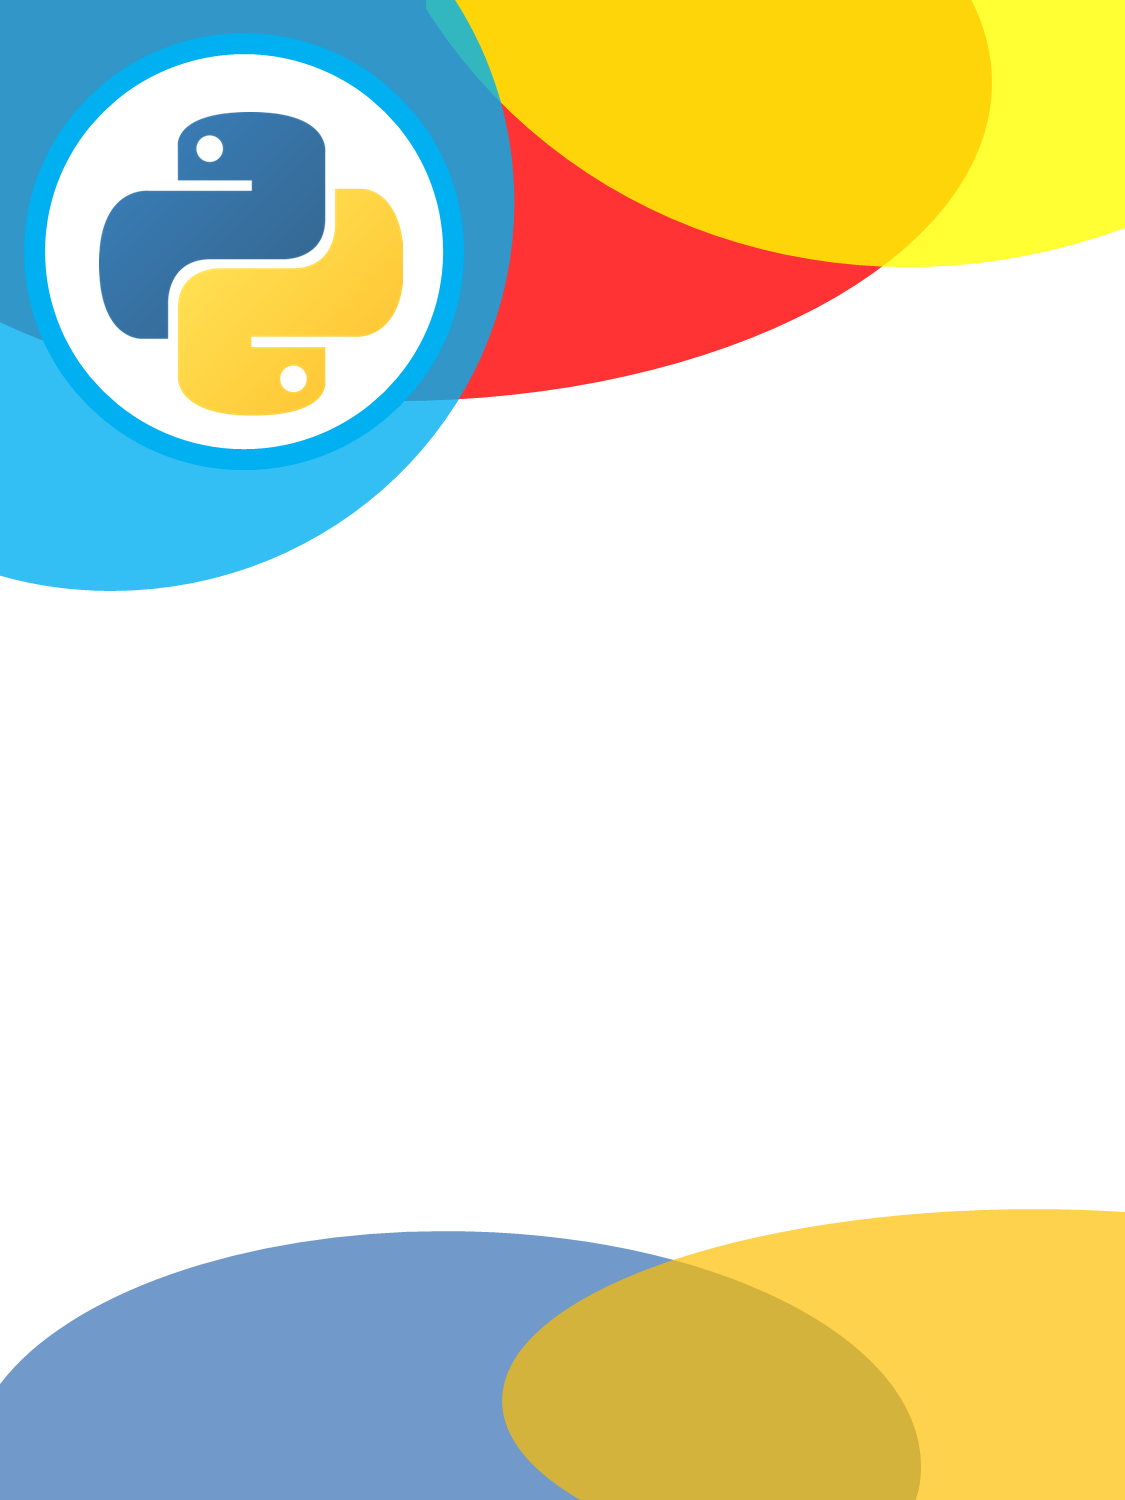
\includegraphics[width=\paperwidth]{capa.png}}; %Capa Imagem A4 21x29.7
\draw[anchor=north] (midpoint) node [fill=ocre!30!white,fill opacity=0.6,text opacity=1,inner sep=1cm]{\Huge\centering\bfseries\sffamily\parbox[c][][t]
        {\paperwidth}
        {\centering Introdu\c{c}\~{a}o \`{a} Linguagem Python\\[5pt] % Titulo Livro
{\Large Paradigmas de Linguagens de Programa\c{c}\~{a}o}\\[20pt] % Subtitle
{\huge \color{blue} Rômulo Souza Fernandes}\\ % Autor nome
{\huge  \color{blue}  Ausberto S. Castro Vera}\\
{\small \today}
}}; % Autor nome
\end{tikzpicture}};
\end{tikzpicture}
\vfill

\endgroup
 
%----------------------------------------------------------------------------------------
%	COPYRIGHT PAGE
%----------------------------------------------------------------------------------------

\newpage
~\vfill
\thispagestyle{empty}

\noindent Copyright \copyright\  \the\year{} Rômulo Souza Fernandes e Ausberto S. Castro Vera\\ % Copyright notice

\noindent \textsc{UENF - Universidade Estadual do Norte Fluminense Darcy Ribeiro}\\ % Universidade

\noindent \textsc{CCT - Centro de Ci\^{e}ncia e Tecnologia}\\ % Centro
\noindent \textsc{LCMAT - Laborat\'{o}rio de Matem\'{a}ticas}\\ % Laboratorio
\noindent \textsc{CC - Curso de Ci\^{e}ncia da Computa\c{c}\~{a}o}\\ % Curso

%\input{autor.tex} \\

\noindent \textit{Primeira edi\c{c}\~{a}o, Setembro 2022} % Printing/edition date

%----------------------------------------------------------------------------------------
%	TABLE OF CONTENTS
%----------------------------------------------------------------------------------------

\chapterimage{sumario01.jpg} % Table of contents heading image

\pagestyle{empty} % No headers

\addtocontents{toc}{\protect{\pdfbookmark[0]{\contentsname}{toc}}}
\tableofcontents % Print the table of contents itself

\cleardoublepage % Forces the first chapter to start on an odd page so it's on the right

\pagestyle{fancy} % Print headers again

%----------------------------------------------------------------------------------------
%	PART
%----------------------------------------------------------------------------------------
%\part{Part One}

%----------------------------------------------------------------------------------------
%	CHAPTERS
%----------------------------------------------------------------------------------------
\chapterimage{capitulo01.jpg} % Chapter heading image
% Prof. Dr. Ausberto S. Castro Vera
% UENF - CCT - LCMAT - Curso de Ci\^{e}ncia da Computa\c{c}\~{a}o
% Campos, RJ,  2022
% Disciplina: Paradigmas de Linguagens de Programa\c{c}\~{a}o
% Aluno: Rômulo Souza Fernandes



\chapter{ Introdução}

Segundo \cite{Borges2014}, o Python é uma linguagem orientada a objetos de alto nível, que possui uma sintaxe simples e objetiva, assim colaborando para a fácil compreensão do código-fonte e permitindo que a linguagem seja produtiva. O Python contém várias estruturas de alto nível, como hora, data, dicionários, listas, complexos, entre outras estruturas. Contém um amplo conjunto de módulos disponíveis para utilização, frameworks que podem ser acrescentados, ferramentas de outras linguagens atuais, como persistência, unidades de teste, geradores, introspecção e metaclasse, além de ter disponíveis diversas bibliotecas, como IPython, Matplotlib, mIPy, NumPy, Pandas, SciPy, ScraPy, entre outras bibliotecas conhecidas.

O Python é uma linguagem multiparadigma, suportando a programação orientada a objetos, modular e funcional. A linguagem Python foi criada na Holanda, no ano de 1990, por Guido van Rossum, no Instituto Nacional de Pesquisa para Matemática e Ciência da Computação. \cite{Borges2014}

A linguagem Python é de código aberto, porém o criador Guido van Rossum possui a função central de decidir a evolução da linguagem. O Python se popularizou e se tornou a linguagem de desenvolvimento de aplicações mais indicada para iniciantes, assim sendo aconselhada como primeira linguagem de programação. \cite{Perkovic2016}

%\begin{quote}

%\end{quote}


\section{História da linguagem Python}

O intuito de Guido van Rossum era criar uma linguagem que pudesse suprir suas exigências, assim criando o Python, com base na linguagem ABC, mas solucionando os problemas encontrados por ele na linguagem. O Python tinha como usuários principais os engenheiros e físicos.


A seguir um pouco da história da linguagem Python, baseados em \cite{Perkovic2016} e \cite{Borges2014} :
\begin{itemize}
  \item O Holandês Guido van Rossum foi o autor principal da linguagem Python. O autor trabalhava no CWI (Centrum Wiskunde \& Informatica), localizada em Amsterdã na Holanda.
  \item  O nome Python não veio da espécie de serpente e sim do seriado de comédia preferido do autor da linguagem, chamado Monty Python's Flying Circus.
  \item A versão 0.9.0 do Python foi lançado em 1991, incluindo manipulação de exceções, classes, listas e strings. Incluía também alguns aspectos de programação funcional como lambda, maps, filter e reduce.
  \item  No ano de 1995, o autor da linguagem continuou seu trabalho sobre Python na Corporation for National Research Initiatives (CNRI) em Reston, Virginia, USA.
  \item  Em Maio de 2000, Guido van Rossum e o grupo de desenvolvimento do Python se mudaram para BeOpen.com, assim formando a equipe BeOpen PythonLabs.
  \item A versão 1.6 do Python foi lançada em 5 de setembro de 2000.
  \item A versão 2.0  do Python foi lançada em 16 de outubro de 2000.
  \item A versão 3.0 do Python foi lançada em 3 dezembro de 2008.
  %\item A última versão lançada do Python é a versão 3.12, lançada em 4 de setembro de 2022
\end{itemize}

%Algumas linguagens s\~{a}o consideradas  tradicionais e outras s\~{a}o consideradas modernas (ver Fig.\ref{afp}). Devemos observar aqui, que a inclus\~{a}o de qualquer figura, significa que ela deve ser referenciada em algum lugar do texto
%   \begin{figure}[H]
	%   \begin{center}
     %   \caption{Logos da Linguagem Python} \label{ling1}
      %  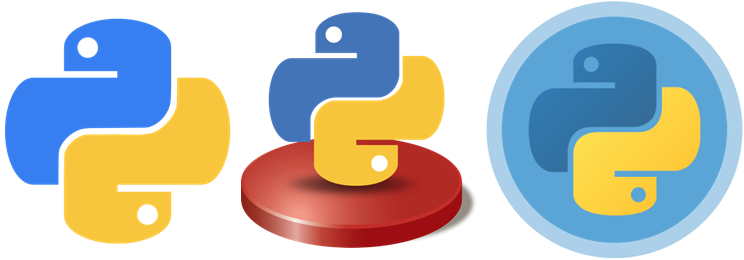
\includegraphics[width=12cm]{Python01.png} \\
       % {\tiny \sf Fonte: O autor deste trabalho }
    %\end{center}
   %\end{figure}

%Algumas figuras s\~{a}o criadas o elaboradas pelo mesmo autor, neste caso, deve-se escrever como fonte "O autor", "Os autores", etc. Figuras que incluam imagens de outras fontes deve-se especificar claramente, indicando o link o referencia correspondente, por exemplo, uma imagem que aparece em \cite[p. 93]{Sprankle2012}, \'{e} mostrada na Fig.\ref{afp} e a fonte deve ser indicada na parte inferior da figura.
   %\begin{figure}[H]
    %\begin{center}
        %\caption{Algoritmo, Diagrama de fluxo, e Pseudo-código} \label{afp}
        %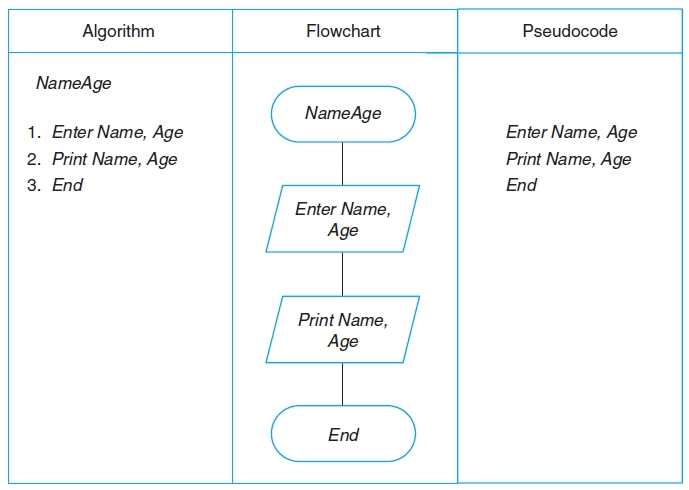
\includegraphics[width=10cm]{afp.jpg} \\
        %{\tiny \sf Fonte: \cite[p. 93]{Sprankle2012} }
    %\end{center}
   %\end{figure}

   \section{Áreas de Aplicação da Linguagem}
   O Python está entre as linguagens de programação mais utilizadas no mundo, é muito utilizado por usuários individuais, mas sua aplicação se estende para empresas reais. A natureza do Python é de propósito geral, assim tornando a linguagem aplicável em quase todas as áreas. Como a IBM, Seagate e Hewlett-Packard, que utilizam o Python para testes de hardware, o Yahoo! e Google usam a linguagem em serviços de Internet, já a empresa Industrial Light and Magic e outras empresas de filmes utilizam o Python na produção de animações. Entre todas as aplicações para o Python atualmente, o ponto em comum é que a linguagem é usada em todo o espectro, em questão de domínios de aplicação. \cite{Lutz2007}

        \subsection{Big Data}
        Atualmente o Python é uma das melhores linguagens de programação para trabalhar com Big Data. Um dos motivos dessa preferência de uso é o suporte avançado de inúmeras bibliotecas e frameworks, muitas das bibliotecas são voltadas para lidar com Big Data, dando suporte e auxiliando na implementação de algoritmos de Machine Learning e Data Analytics. Abaixo algumas das bibliotecas de software livre:
        \begin{itemize}
        	\item SciPy: Utilizada para computação técnica e computação científica, possibilita a interpolação, otimização, integração e modificação de dados utilizando funções especiais, álgebra linear, etc.
        	
        	\item NumPy: Utilizada para computação numérica para dados com formas de grandes matrizes multidimensionais e Arrays. A biblioteca também oferece diversas funções matemáticas de alto nível, para manipular os dados com transformada de Fourier, álgebra linear, processamento de números aleatórios, etc.
        	
        	\item Scikit-learn: Utilizada para Machine Learning, relacionada a vários algoritmos de regressão, clustering e classificação. Pode ser utilizada também em conjunto com outras bibliotecas, como a NumPy e SciPy.
        	
        	\item Pandas: Utilizada para análise e manipulação de dados, oferece diversas estruturas de dados e operações para manipulação de dados, no formato de séries temporais e tabelas numéricas. A biblioteca também dispõe de diferentes ferramentas para gravar e ler dados, entre estruturas de dados na memória e diferentes formatos de arquivo.
        \end{itemize}
        
        O Python possui uma sintaxe simples, possibilitando uma fácil leitura do código, assim tanto os iniciantes quanto os desenvolvedores experientes, podem se concentrar melhor no objetivo, ao invés de se desgastar se concentrando nas nuances técnicas da linguagem que está utilizando. Sendo assim, o Python é a linguagem preferida dos Cientistas de dados e Engenheiros de Big Data. 
        
        A linguagem Python é extremamente flexível, permitindo finalizar mais trabalhos com menor número de linhas de código. O Python também é escalável na manipulação de dados em grandes quantidades, sendo um ponto muito importante quando se trata de Big Data. Comparando o Python com outras linguagens de programação utilizadas em Big Data Analytics, como R e Java, elas não são tão escaláveis e flexíveis como o Python, onde havendo um aumento no volume de dados, o Python sem dificuldades pode aumentar a velocidade de processamento dos dados, sendo uma tarefa complicada para fazer em R ou Java. \cite{McKinney2019}

        \subsection{Orientação a objetos}  
        O Python é uma linguagem multiparadigma, suportando diferentes abordagens de programação, um jeito de solucionar problemas de programação é criar objetos, esse método é conhecido como Programação Orientada a Objetos(POO) e a orientação a objetos é um dos paradigmas da linguagem Python, com isso, a criação de objetos e classes é mais simples. 
        
        No Python os dados são guardados em objetos, em outras linguagens, determinados tipos são guardados na memória, não em entidades abstratas como objetos. A programação orientada a objetos é um importante método de organizar e desenvolver códigos, focando em criar códigos reutilizáveis. \cite{Lutz2007}
        
        No Python, a programação orientada a objetos possui alguns pontos importantes, baseados no mesmo autor citado no parágrafo anterior: 
        \begin{itemize}
        	\item Encapsulamento: Restrição ao acesso de métodos e atributos de uma classe, evitando que os dados sejam alterados diretamente, na linguagem Python existe apenas o private e public.
        	
        	\item Métodos: São funções definidas no corpo da classe. Utilizados para definir o comportamento do objeto. 
        	
        	\item Objeto: É a instância de uma classe. Somente a definição do objeto é definida no momento em que a classe é estabelecida. Consequentemente nenhum espaço de memória é alocado.
        	
        	\item Classe: Juntam as funcionalidades de um certo objeto, servindo como um modelo.
        	
        	\item Polimorfismo: É a capacidade de utilizar uma interface para vários tipos de dados. Possibilitando que o objeto possua o poder de assumir diversas formas. 
        	
        	\item Herança: Cria uma classe nova que será descendente e irá utilizar particularidades de outra classe já existente, sem realizar modificações na mesma.
        	 
        	
        \end{itemize}


        \subsection{Pentest} 
        O Python está entre as melhores linguagens para pentest e segurança da informação, isso é devido a grande quantidade de bibliotecas, ferramentas, frameworks, por ter versatilidade e ser multiplataforma, entre outros pontos que tornam o Python uma das melhores linguagens para essa aplicação, como ter um código de fácil leitura e sintaxe simples. A linguagem é usada para diversas finalidades dentro do processo, possibilitando que as soluções sejam vinculadas e automatizadas sem dificuldades, como decodificar e enviar pacotes, varrer redes e portas, analisar malwares, acessar servidores, etc, com base em \cite{Moreno2018} e \cite{Seitz2015}.
        
        Como citado, a linguagem Python possui uma grande diversidade de ferramentas, de acordo com os mesmos autores citados no parágrafo anterior, essas são algumas das ferramentas disponíveis:
        \begin{itemize}
        \item Análise de malware:
        	\begin{itemize}
        		\item Exefilter: Utilizada para filtrar tipos de arquivos para páginas web e e-mails, podendo detectar diversos tipos de arquivos e apagar o conteúdo ativo.
        		
        		\item PyClamAV: Acrescenta a detecção de vírus maliciosos nas ferramentas do Python.
        		
        		\item Pyew: Utilizada geralmente para analisar malwares, o pyew desmonta e edita hexadecimais de linha de comando.
        	\end{itemize}
        
        \item Utilitários de rede:
        	\begin{itemize}
        		\item Dpkt: Utilizado para gerar e analisar pacotes de dados utilizando definições do protocolo TCP/IP.
        		\item Spoodle: Usado para verificar subdomínios e vulnerabilidade.
        		\item Knock Subdomain Scan: utilizado para retornar a lista de subdomínios do domínio de destino através da técnica de lista de palavras.
        	\end{itemize}
        
        \item Explorar bibliotecas:
        	\begin{itemize}
        		\item Scapy: É uma biblioteca e ferramenta de processamento de pacotes, podendo decodificar diversos protocolos, enviar pela rede, capturar e combinar respostas e solicitações. Oferece funções como as oferecidas pelo Tcpdump, Wireshark e Nmap, também oferece acesso programático.
        		
        		\item Python Nmap: Usado para analisar os resultados da varredura do Nmap e lançar ataques particularizados contra hosts específicos.
        		
        		\item Monda: O Monda é um depurador de imunidade, que auxilia no desenvolvimento de programas de exploração.
        		
        	\end{itemize}
        
        \item Forense
        	\begin{itemize}
        		\item Rekall: O Rekall é um framework criado pelo Google para realizar varreduras e análises de memória.
        		
        		\item LibForensics: É uma biblioteca para desenvolvimento de aplicativos Forenses digitais
        		
        		\item Aft: É um pacote de ferramentas forenses voltado para Android.
        		
        	\end{itemize}
        \end{itemize}
    
   
    	

\chapterimage{capitulo.jpg} % Chapter heading image
% Prof. Dr. Ausberto S. Castro Vera
% UENF - CCT - LCMAT - Curso de Ci\^{e}ncia da Computa\c{c}\~{a}o
% Campos, RJ,  2022
% Disciplina: Paradigmas de Linguagens de Programa\c{c}\~{a}o
% Aluno: Rômulo Souza Fernandes


\chapter{ Conceitos básicos da Linguagem Python}

Neste capítulo é apresentado alguns conceitos básicos da linguagem de programação Python, como Variáveis, constantes e tipos de dados básicos aceitos pela linguagem, que são inteiro, ponto flutuante, booleano, string e lista. Alguns dos livros indicados para iniciar o estudo sobre a linguagem de programação Python são:  \cite{Lutz2007}, \cite{Perkovic2016}, \cite{Severance2016}, que foram os mesmos livros usados como base para escrever grande parte desse e outros capítulos.

    %%%%%%%%=================================
    \section{Variáveis e constantes}
    %%%%%%%%=================================
	De acordo com \cite{Severance2016} o Python possui um ótimo recurso que é a manipulação de variáveis, essas variáveis são nomes atribuídos a valores, que possuem como propósito armazenar valores de forma que mais tarde possam ser recuperados. 
	Para criar variáveis é necessário fazer uma declaração por atribuição e atribuir valores a essas novas variáveis. 
	\begin{lstlisting}
	>>> texto = 'Hello, world!'
	>>> pi = 3,14159265
	>>> numero = 1500
	\end{lstlisting}
	No exemplo acima podemos observar a declaração por atribuição de 3 variáveis diferentes. A primeira está atribui uma string para uma variável chamada texto, a segunda variável atribui o valor 3,14 que é conhecido como Pi e a variável possui o nome pi. Já a terceira variável numero está recebendo o valor 1500, também por atribuição. Os usuários tem uma grande liberdade na hora de escolher os nomes das variáveis, apenas não sendo possível usar palavras reservadas da linguagem como nome de uma variável.
	
	As constantes na linguagem Python, diferente de outras linguagens de programação, não podem ser criadas de forma que seu valor não seja alterado. Na documentação existem algumas orientações caso o usuário queira criar uma constante com sintaxe de variável, uma delas é que todas as letras da variável que será utilizada como constante, deveram ser maiúsculas, em casos do nome desejado possuir espaço, deverá ser utilizado underline.
	\begin{lstlisting}
	>>> PRECO = 5
	>>> PRECO_PRODUTO = 2
	\end{lstlisting}
	O exemplo acima é o padrão recomendado pela documentação do Python.

    %%%%%%%%=================================
    \section{Tipos de Dados Básicos}
    %%%%%%%%=================================
	A linguagem de programação Python é de tipagem dinâmica, com isso não é preciso declarar o tipo de variável, o tipo será definido através do valor que a variável receber, isso possibilita que o tipo mude no decorrer da execução do programa. Vamos falar sobre esses tipos de dados a seguir, com base nos autores \cite{Lutz2007}, \cite{Perkovic2016}, \cite{Severance2016}.
	
			\subsection{Inteiro}
			De acordo com o autor \cite{Perkovic2016}, o tipo inteiro ou \textit{int} representa caracteres numéricos inteiros positivos e negativos. Como já informado no texto anteriormente, na linguagem Python não é necessário informar o tipo da variável na sua declaração, o exemplo abaixo deixará isso mais claro.
			\begin{lstlisting}
   >>> n1 = 5
   >>> n2 = 10
   >>> soma = n1 + n2
   >>> print(soma)	
   >>> print(type(soma))		
   15
   <class 'int'>
			\end{lstlisting}
		
			\subsection{Ponto Flutuante}
			Com base no \cite{Perkovic2016}, \textit{float} ou ponto flutuante é um tipo de dado usado para os números reais, pois eles possuem casas decimais, explicando melhor, são números com vírgula, como por exemplo peso ou altura. Em uma expressão numérica, se um dos valores for um \textit{float}, o resultado da expressão será um \textit{float}, o exemplo abaixo irá demonstrar.
			\begin{lstlisting}
   >>> #exemplo utilizando ponto flutuante
   >>> peso = 1.77
   >>> altura = 62.50
   >>> print(type(peso))
   >>> print(type(altura))
   <class 'float'>
   <class 'float'>
   
   >>> #exemplo utilizando 1 ponto flutuante e 1 inteiro
   >>> a = 5
   >>> b = 2.5
   >>> soma = 5 + 2.5
   >>> print(soma)
   >>> print(type(resultado))
   7.5
   <class 'float'>
			\end{lstlisting}
		
			\subsection{Booleano}
			Segundo \cite{Perkovic2016}, o booleano é um tipo de dado lógico, utilizado parar armazenar valores lógicos, que no Python pode ser representado pelo valor True ou False. O True significando que o valor é verdadeiro e False significa que seu valor é falso. Seguimos com alguns exemplos do tipo de dado lógico booleano.
			\begin{lstlisting}
   >>> x = false
   >>> print(type(x))
   <class 'bool'>
   
   >>> #operacoes logicas
   >>> a = 10 < 5
   >>> print(a)
   False
   
   >>> b = c = 5
   >>> print(b <= c and c <= b)
   True
   
			\end{lstlisting}
     %%%........................
            \subsection{String}
     %%%........................
            Com base no autor \cite{Severance2016}, uma string é uma sequência de caracteres imutável, não permitindo alterar uma string que já existe. É classificado como um item de dado simples. Para o Python, uma string é um array de caracteres ou qualquer grupo de caracteres escritos entre doble aspas ou aspas simples, por exemplo:
    \begin{lstlisting}
    >>> #Aspas simples
    >>> menssagem1 = 'Hello, World'
    >>> print (menssagem1)  
    Hello, World
    
    >>> #Aspas duplas
    >>> mensagem2 = "O dia esta chuvoso"
    >>> print (menssagem2)
    O dia esta chuvoso
    \end{lstlisting}
			
    \begin{itemize}
      \item \textit{Concatenação de strings}\\
            A união de strings é chamado de concatenação, isso pode ser feito utilizando o operador +, que possui essa função de concatenar quando usado com operandos do tipo string. O comprimento de uma string pode ser calculado utilizado o operador \texttt{len(string)}.
     \begin{lstlisting}
    >>> # concatenando 2 strings
    >>> moto = "Titan " + "150 ESD"
    >>> print (moto)
    Titan 150 ESD
    
    >>> print (len(moto))
    13
    \end{lstlisting}

      \item \textit{Operador de indexação}\\
      Utilizando o operador de indexação é possível acessar os caracteres um por um, utilizando o operador colchetes, o número dentro do colchetes é denominado index, usado para indicar a posição do caractere da variável e atribuir esse caractere à uma variável.
      Existem duas formas de indexar os caracteres de um string em Python:\\
      \begin{description}
        \item[Index com inteiros positivos] indexando a partir da esquerda, começando com 0, sendo o 0 o index do primeiro caractere da sequência.
        \item[Index com inteiros negativos] indexando a partir da direita, começando com -1, sendo -1 o último elemento da sequência, -2 sendo o penúltimo elemento da sequência, e assim sucessivamente.
      \end{description}

     \begin{lstlisting}
     >>> #Inteiro positivo
     >>> moto = 'titan'
     >>> letra = moto[0]
     >>> print(letra)
     t
     
     >>>#inteiro negativo
     >>>moto = 'titan'
     >>>letra = moto[-1]
     >>>print(letra)
     n
        \end{lstlisting}


      \item \textit{Operador de Fatias}\\
      O operador de acesso a itens de forma individual, também pode ser usado como operador de fatias, podendo assim extrair uma fatia inteira (subsequência) de caracteres de uma string. O operador de Fatias dispõe de três sintaxes:\\
      \texttt{sequencia[ inicio ]}\\
      \texttt{sequencia[ inicio : fim ]} \\
      \texttt{sequencia[ inicio : fim : step ]}\\
      onde \texttt{início, fim} e \texttt{step} são números inteiros.
     \begin{lstlisting}
    >>> sequencia = 'Linguagem Python'
    >>> print(sequencia[0:9])
    Linguagem
    
    >>> print(sequencia[0:9:8])
    Lm
        \end{lstlisting}

    \end{itemize}

			\subsection{Lista}
			Segundo o autor \cite{Severance2016}, lista é uma sequência de objetos, diferente de uma string onde os valores são caracteres, na lista esses valores podem ser de qualquer tipo, até mesmo outras listas. Outra característica da lista que difere de uma string é que as listas são mutáveis, assim permitindo que o seu conteúdo seja modificado em qualquer momento, esse conteúdo das listas é chamado de elementos ou itens. Para criar uma lista é necessário colocar seus elementos apenas entre colchetes ou entre aspas dentro dos colchetes caso os elementos sejam caracteres.
			
			\begin{lstlisting}
	['verde ', 'amarelo', 'azul']
	[1, 2, 3, 4, 5]
			\end{lstlisting}
		A primeira lista do exemplo é formada por três strings, enquanto a segunda é formada por cinco números inteiros. Como já citado, é possível criar uma lista com elementos de tipos diferentes, como no exemplo a seguir, onde a lista contém uma lista, uma string, um float e um inteiro..
			
			\begin{lstlisting}
	[[1, 2], 'amarelo', 3.14, 100]
			\end{lstlisting}
		
		Também é possível atribuir valores de uma lista a variáveis.
		\begin{lstlisting}
	>>> numeros = [1, 2, 3, 4, 5]
	>>> cores = ['verde ', 'amarelo', 'azul']
	>>> lista_vazia = []
	
	>>> print(numeros, cores, lista_vazia)
	[1, 2, 3, 4, 5] ['verde ', 'amarelo', 'azul'] []
		\end{lstlisting}
	
	O acesso de elementos de uma lista é da mesma forma que o acesso de caracteres de uma string, o exemplo a seguir demonstra o funcionamento, o valor dentro dos [] é o índice.
	\begin{lstlisting}
		>>> print(cores[1])
		amarelo
	\end{lstlisting}
	Como as listas são mutáveis, é possível alterar seu conteúdo, atribuindo novos valores a itens ou mudando a ordem desses itens. A seguir temos um exemplo se como realizar essa alteração, observe que os [] a esquerda na atribuição significa o elemento que será alterado.
	\begin{lstlisting}
	>>> numeros = [1, 2, 3, 4, 5] 
	>>> numeros[0] = 6
	>>> print(numeros)
	[6, 2, 3, 4, 5]
	\end{lstlisting}

	\begin{itemize}
	\item {Operações com Listas}
	
	Novamente como nas strings, o + é o operador utilizado para concatenar listas e o * repete a lista determinada a quantidade de vezes desejada.
	
	\begin{lstlisting}
	>>> #concatenacao
	>>> numeros = [1, 2, 3]
	>>> cores = ['verde ', 'amarelo', 'azul']
	>>> concatena = numeros + cores
	>>> print(concatena)
	[1, 2, 3, 'verde ', 'amarelo', 'azul']
	
	>>> #repeticao de lista
	>>> print([1,2,3] * 3)
	[1, 2, 3, 1, 2, 3, 1, 2, 3]
	
	>>> print(['vermelho'] * 3)
	['vermelho', 'vermelho', 'vermelho']
	\end{lstlisting}

	\end{itemize}
     %%%%%%%%=================================
    \section{Tipos de Dados de Coleção}
    %%%%%%%%=================================


     %%%........................
            \subsection{Tipos Sequenciais}
     %%%........................
	 Com base em \cite{Severance2016}, as tuplas são sequências de valores parecidas com a lista, com a diferença que as tuplas são imutáveis, porém é possível cria uma tupla que contenha objetos mutáveis, um exemplo seria uma lista. Os valores para se armazenar podem ser de todos os tipos, são indexados usando números inteiros. A tupla é uma sequência de valores separados por vírgulas.
	\begin{lstlisting}
	>>> A = 123, 456, 'ola mundo'
	>>> A[1]
	456	
	\end{lstlisting}
	Para aninhar tuplas é necessário envolver por parênteses, permitindo que possam ser lidas corretamente. O uso de parênteses não é obrigatório para a criação de tuplas, apenas para tuplas dentro de expressões. A seguir temos uma demonstração.
	\begin{lstlisting}
	>>> B = A, (1, 2, 3)
	>>> B
	((123, 456, 'ola mundo'), (1, 2, 3))
	\end{lstlisting}
	

     %%%........................
            \subsection{Tipos Conjunto}
     %%%........................
	Segundo o autor \cite{Perkovic2016}, no Python um conjunto ou \textit{set} é uma coleção de itens fora de ordem, não podendo incluir itens duplicados. Desde que sejam imutáveis, as chaves podem ser de qualquer tipo. A linguagem oferece diferentes formas eficazes para criação e manipulação desses \textit{sets}, assim admitindo operadores para interseção, união, inclusão em conjunto, diferença simétrica, entre outros operadores disponíveis. Os \textit{sets} são definidos utilizando a mesma sintaxe utilizada para os conjuntos matemáticos, sendo itens separados por virgula e em sequência, sendo delimitados por chaves.
	\begin{lstlisting}
	>>> #criando e printando um conjunto
	>>> anotacao = {'123-456-789', '987-654-321',}
	>>> print(anotacao)
	{'987-654-321', '123-456-789'}
		
	>>> #verificando o tipo
	>>> type(anotacao)
	<class 'set'>
	\end{lstlisting}
	
     %%%........................
            \subsection{Tipos Mapeamento}
     %%%........................
	Com base no autor \cite{Severance2016}, na linguagem Python o dicionário é o único tipo de mapeamento nativo, seu funcionamento é como de uma lista, porém é mais geral. Explicando melhor, nas listas o índice necessariamente é um inteiro, já no dicionário o índice pode ser quase todos os tipos de dados. O dicionário é um mapeamento entre um conjunto de valores e índices, assim a chave que é o índice, é usado para localizar um valor. O dicionário é indicado por \textit{dict}.
		\begin{lstlisting}
  >>> #criando e printando um dicionario
  >>> dic = {'gasolina': 5.30, 'alcool': 4.30, 'GNV': 4.50}
  >>> print(dic)
  {'gasolina': 5.3, 'alcool': 4.3, 'GNV': 4.5}
  
  >>> #item que localiza pela chave 'GNV'
  >>> print(dic['GNV'])
  4.5
	\end{lstlisting}
	Como mostrado no exemplo acima, a chave 'GNV' sempre irá localizar o valor 4.5, assim mostrando também que a ordem dos itens não interfere.

    %%%%%%%%=================================
    \section{Estrutura de Controle e Funções}
    %%%%%%%%=================================
	
     %%%........................
            \subsection{O comando IF}
     %%%........................
			O \textit{if} é uma estrutura de controle, sendo de decisão fundamental, permitindo a execução de blocos de códigos alternativos, se baseando em condições.
			\begin{lstlisting}
	>>> if A > 0
	>>> 	print('A e um numero positivo')
	
			\end{lstlisting}
			 Depois da declaração textit{if} temos uma expressão booleana, essa expressão é a condição. Como vemos no exemplo acima, a declaração termina com o símbolo de dois pontos (:) e a linha após o textit{if} devem ser indentadas. A condição lógica sendo verdadeira, logo a declaração é executada, caso seja falsa, a condição é ignorada.
			 
			 As declarações que se alongam por mais de uma linha e consistem em uma linha de cabeçalho e um bloco indentado, são chamadas de extit{declarações compostas}. O número de declarações possíveis não tem um limite, porém é obrigatório que tenha no mínimo uma. 
			 
			 \begin{itemize}
			 	\item \textit{Execução alternativa}
			 	
			 	 A \textit{Execução alternativa} é a segunda forma de declarar um \textit{if}, nessa declaração existem duas possibilidades e a sua condição, que irá determinar qual delas será executada. Abaixo temos uma demonstração se o número é par ou ímpar.
			 	 \begin{lstlisting}
	>>> if A%2 == 0
	>>>		print('A e Par')
	>>> else:
	>>>		print('A e Impar')

			 	 \end{lstlisting}
				\item \textit{Condição encadeada}
				
				A condição encadeada é um jeito de expressar uma lógica computacional, utilizada quando existe mais de uma possibilidade e necessitamos de mais de duas ramificações. 
				
				\begin{lstlisting}
	>>> if n1 < n2:
	>>>	print('n1 e menor que n2')
	>>> elif n1 > n2:
	>>>	print('n1 e maior que n2)
	>>> else:
	>>>	print('n1 e n2 sao iguais')
					
				\end{lstlisting}
			
				\item \textit{Condição aninhadas}
				Também podemos escrever com 3 ramos, assim a condição passará a ser aninhada, vamos exemplificar na demostração abaixo.
					\begin{lstlisting}
	>>> if n1 == n2:
	>>>	print('n1 e n2 sao iguais')
	>>> else:
	>>>	if p1 < p2:	
	>>>	    print('n1 e menor que n2)
	>>>	else:
	>>>	    print('n1 e maior que n2')
					
				\end{lstlisting}
			 \end{itemize}
			  
      %%%........................
            \subsection{Laço FOR}
     %%%........................
	Segundo \cite{Severance2016} podemos criar um laço definido utilizando uma declaração \textit{for}, quando temos um conjunto de itens para iterar. É chamado de laço definido pois irá iterar sobre uma lista de itens até que o número de iterações seja o mesmo de itens da lista. Abaixo temos um exemplo de declaração \textit{for}, onde o \textit{for} e \textit{in} são palavras-chave reservadas do Python, colegas e colega são variáveis, colega em específico é uma \textit{variável de iteração} do laço \textit{for}, que percorre o conteúdo da variável amigos, mudando a cada iteração, assim controla quando o laço deve finalizar.
	\begin{lstlisting}
	>>> colegas = ['Marta', 'Lucas', 'Diego']
	>>> for colega in colegas:
	>>>	print('Bom dia', colega)
	Bom dia Marta
	Bom dia Lucas
	Bom dia Diego
		
	\end{lstlisting}
	Para o Python, a variável colegas é considerada uma lista contendo 3 cadeias de caracteres e um laço \textit{for}, que percorrerá a lista e executará o corpo 1 vez para cada palavra da lista, por isso a saída mostra a mensagem para todo os colegas da lista.
     %%%........................
            \subsection{Laço WHILE}
     %%%........................
	De acordo com \cite{Severance2016} a linguagem Python oferece vários recursos para tornar a automatização de tarefas repetitivas mais fácil. No Python, o \textit{while} é uma forma de iteração. A seguir temos uma demonstração de uso do \textit{while} e também podemos perceber novamente a clareza da sintaxe do Python, a declaração pode ser lida como uma frase usual.
	\begin{lstlisting}
	>>> x = 2
	>>> while x > 0:
	>>>	print(x)
	>>>	x = x-1
	>>> print('Go!!!')
		
	\end{lstlisting}
	O fluxo de execução é, analisar a condição, assim retornando o valor \textit{True} ou \textit{False}, caso a condição seja falsa, sai da declaração e segue para as próximas declarações, já caso seja verdadeira, executa o bloco \textit{while} e retorna para o primeiro passo, que é analisar a condição. O bloco de instruções também pode ser chamado de \textit{laço}, visto que o terceiro e último passo retorna para o primeiro. A cada vez que as instruções internas de um laço são executadas, chamamos de \textit{iteração}. A \textit{variável de iteração} é a variável que tem seu valor modificado a cada execução do laço, assim controlando quando o laço deve acabar. Podemos chamar uma declaração \textit{while} de laço indefinido, pois a declaração continua iterando até que uma das condições seja falsa.
	
	
    %%%%%%%%======================
    \section{Módulos e pacotes}
    %%%%%%%%======================



       %%%........................
            \subsection{Módulos}
     %%%........................
	Os módulos são arquivos que contém definições e instruções, são utilizados em uma execução ou script interativa do interpretador. Essas definições podem ser importadas para o módulo principal ou outro módulo. O arquivo tem mesmo nome do módulo porém com o acrescimo do \textit{.py}. O próprio Python possui uma variedade de módulos na sua biblioteca padrão. Após a importação do módulo podemos usar as instruções e definições que estão contidas nele. Abaixo um exemplo prático.
	\begin{lstlisting}
		>>> # Fibonacci numbers module
		>>> def fib(n):    # write Fibonacci series up to n
		>>> a, b = 0, 1
		>>> while a < n:
		>>> print(a, end=' ')
		>>> a, b = b, a+b
		>>> print()
		
		>>> def fib2(n):   # return Fibonacci series up to n
		result = []
		>>> a, b = 0, 1
		>>> while a < n:
		>>> result.append(a)
		>>> a, b = b, a+b
		return result
		
	\end{lstlisting}


          %%%........................
            \subsection{Pacotes}
     %%%........................






    Código fonte para a linguagem Python:
    \begin{lstlisting}
    number_1 = int(input('Ingresse o primeiro numero: '))
    number_2 = int(input('Ingresse o segundo numero: '))

    # Soma
    print('{} + {} = '.format(number_1, number_2))
    print(number_1 + number_2)

    # Substra\c{c}\~{a}o
    print('{} - {} = '.format(number_1, number_2))
    print(number_1 - number_2)

    # Multiplica\c{c}\~{a}o
    print('{} * {} = '.format(number_1, number_2))
    print(number_1 * number_2)

    # Divis\~{a}o
    print('{} / {} = '.format(number_1, number_2))
    print(number_1 / number_2)
    \end{lstlisting}






% Prof. Dr. Ausberto S. Castro Vera
% UENF - CCT - LCMAT - Curso de Ci\^{e}ncia da Computa\c{c}\~{a}o
% Campos, RJ,  2022
% Disciplina: Paradigmas de Linguagens de Programa\c{c}\~{a}o
% Aluno: Rômulo Souza Fernandes


\chapter{ Programação Orientada a Objetos com Python}

	 Como sabemos, a Programação Orientada a Objetos (POO) é um dos paradigmas da linguagem Python, com base no conceito de classes e objetos. Com isso trás ótimas e poderosas ferramentas que auxiliam no desenvolvimento de softwares seguros e confiáveis, uma dessas ferramentas que auxiliam é a herança, que evita trabalhos repetidos, permite também que o desenvolvedor codifique com maior velocidade, poupando tempo. Esse paradigma é voltado para os objetos desejados pelos desenvolvedores, ao contrário da lógica essencial para manipular. A seguir vamos explicar e demonstrar cada conceito da Programação Orientada a Objetos.

   %%%%%%%%======================
    \section{Classes e Objetos}
    %%%%%%%%======================
    
	 No Python uma entidade é representada por uma abstração computacional chamada objeto, que possui os atributos, são as qualidades e os métodos que são as ações que a entidade pode fazer. Na orientação a objetos, classe é a estrutura básica, simbolizando o tipo de um objeto, assim definindo o que o objeto pode realizar e suas características. A seguir temos um exemplo simples de como definir uma classe:
	 \begin{lstlisting}
   class NomedaClasse:
   <statement-1>
   .
   .
   .
   <statement-N>
	 \end{lstlisting}
	  
	 Para que o objeto permaneça na memória é preciso de no mínimo uma referência, pois o interpretador da linguagem Python tem uma ferramenta de limpeza que exclui todos os objetos que não possuem referência, essa ferramenta é chamada de coletor de lixo ou \textit{Garbage Collector}, assim que os objetos sem referência são excluídos o \textunderscore\textunderscore \textit{done}\textunderscore\textunderscore(), que é um método especial, é executado.
	 
	Há diversos motivos para o Python aceitar que classes novas sejam definidas por desenvolvedores, um dos motivos é que o programa de aplicação será mais simples de desenvolver, ler, depurar e intuitivo, através das classes projetadas unicamente para essa aplicação. Junto com a possibilidade de criar classes novas é permitido um novo jeito de estruturar um programa de aplicação. O comportamento de uma função é exposto ao usuário, mas sua implementação é encapsulada(ocultada) \cite{Borges2014}. 
	
	A seguir temos uma demonstração de uso do objeto no Python:
	
   \begin{lstlisting}
    stuff = list()
    stuff.append('python')
    stuff.append('chuck')
    stuff.sort()
    print (stuff[0])
    print (stuff.__getitem__(0))
    print (list.__getitem__(stuff,0))
    \end{lstlisting}
	
	Na primeira linha um objeto do tipo \textit{list} é construído, na segunda e terceira linhas do código o método \textit{append()} é chamado, na quarta linha o método \textit{sort()} é chamado, na quinta linha o item da posição 0 é recuperado. 
	
	Na sexta linha o método \textunderscore\textunderscore \textit{getitem}\textunderscore\textunderscore()  com 0 como parâmetro, é chamado na lista \textit{stuff}.
	\begin{lstlisting}
    print (stuff.__getitem__(0))
	\end{lstlisting}

	Na sétima linha mostra como recuperar o primeiro item da lista de uma forma mais detalhada.
	\begin{lstlisting}
    print (list.__getitem__(stuff,0))
	\end{lstlisting}
	
	Neste código o método \textunderscore\textunderscore \textit{getitem}\textunderscore\textunderscore () é chamado na classe \textit{list} e também é passado o item que deve ser recuperado e a lista como parâmetro. As 3 últimas linhas do código percebemos que são semelhantes, porém fazer uso da sintaxe com os colchetes ([ ]) é mais adequado para visualizar um item em uma posição específica da lista \cite{Severance2016}.
	
   %%%%%%%%======================
    \section{Operadores ou Métodos}
    %%%%%%%%======================
	De acordo com o autor \cite{Borges2014}, um método é uma função utilizada para detalhar o comportamento do objeto. Os métodos que conseguem se aplicar aos objetos da classe são expostos ao usuário, mas o modo como essas informações inclusas nos objetos são salvas, é encapsulado, além de encapsular o modo como os métodos das classes estão sendo implementados.
	 
	Um operador é uma chamada para os métodos especiais. Os métodos especiais são caracterizados pelos nomes que possuem um padrão, utilizando 2 sublinhados no começo e 2 no final de cada nome, definindo de que forma os objetos que são derivados da classe devem funcionar em casos específicos, conforme na sobrecarga de operadores.
	
	 Na linguagem de programação Python um objeto é criado com base na classe, usando a atribuição. O construtor dessas classes que é um método especial, entra em execução quando novos objetos são criados. Esse construtor é chamado de \textunderscore\textunderscore \textit{new}\textunderscore\textunderscore(), depois de chamar o construtor para inicializar uma nova instância é chamado o método \textunderscore\textunderscore \textit{init}\textunderscore\textunderscore(). Uma forma da classe definir um método especial \textunderscore\textunderscore \textit{init}\textunderscore\textunderscore() é:
	 \begin{lstlisting}
   def __init__(self):
   self.data = []
	 \end{lstlisting}
	 
	
   %%%%%%%%======================
    \section{Herança}
    %%%%%%%%======================
	A herança é uma grande ferramenta do Python, devido a programação orientada a objetos. Essa ferramenta possui objetivo de facilitar o reaproveitamento de códigos. Organizando as classes definidas pelo usuário é possível reutilizá-las em outros códigos, de forma semelhante como é possível utilizar uma função no desenvolvimento de outra função. Assim novos atributos e métodos podem ser implementados por uma nova classe e ao mesmo tempo a classe pode herdar atributos e métodos de uma classe antiga. Além disso as classes podem ser estendidas em uma classe nova através da herança de classes. 
	
	Existem 2 tipos de heranças, simples e múltipla. Na herança simples a classe pode derivar apenas de uma classe que já existe, diferentemente na herança múltipla a classe deriva de diversas classes que já existem, outra diferença é na ordem de resolução dos métodos, seguindo o algoritmo diamante \cite{Borges2014}.
	
	A seguir uma demonstração de herança simples e herança múltipla: 
	
	\begin{lstlisting}
    # Heranca simples
    class DerivedClassName(BaseClassName):
    <statement-1>
    .
    .
    .
    <statement-N>
		
    # Heranca multipla
    class DerivedClassName(Base1, Base2, Base3):
    <statement-1>
    .
    .
    .
    <statement-N>
	\end{lstlisting}

% Prof. Dr. Ausberto S. Castro Vera
% UENF - CCT - LCMAT - Curso de Ci\^{e}ncia da Computa\c{c}\~{a}o
% Campos, RJ,  2022
% Disciplina: Paradigmas de Linguagens de Programa\c{c}\~{a}o
% Aluno: Rômulo Souza Fernandes



\chapter{ Aplica\c{c}\~{o}es da Linguagem Python}

Neste capítulo será apresentada 5 aplicações completas na linguagem de programação Python, com base nos autores \cite{Perkovic2016}, \cite{Borges2014}, \cite{Severance2016} e \cite{Lutz2007}. Cada caso contém:
\begin{itemize}
  \item Uma breve descrição da aplicação
  \item O código completo da aplicação com comentários explicativos
  \item Imagens dos resultados após a compilação-interpretação do código fonte
\end{itemize}




    \section{Operações básicas}
    
    O código a seguir apresenta algumas operações básicas da matemática que podem ser feitas na linguagem Python, como adição, subtração, multiplicação e divisão. Essas operações serão escolhidas em um menu de opções. 
	\begin{lstlisting}
# Autor: Romulo Souza Fernandes
# E-mail: 00119110559@pq.uenf.br
# Data de criacao: 28/10/22
# Ciencia da Computacao - UENF
# Disciplina: PLP
		
		
continuar_usando = "SIM"
		
while continuar_usando == "SIM":
 # Criando um menu de opcoes
 print("SELECIONE A OPERACAO DESEJADA")
 print("+ para Adicao")
 print("- para Subtracao")
 print("* para Multiplicacao")
 print("/ para Divisao")
		
 # Interacao com o usuario
 operacao = input("\nQual operacao voce deseja realizar? ")
		
 # Criando as operacoes e as apresentacoes de respostas
		
 # Adicao
 if operacao == "+":
  a1 = float(input("\nDigite o primeiro valor: "))
  a2 = float(input("Digite o segundo valor: "))
  adicao = a1 + a2
  print("\nA soma entre", a1, "e", a2, "e:", adicao, "\n")
  print("*"*33, "\n")
  continuar_usando = input("Gostaria de fazer outra operacao? 
  ").upper()
  print("*"*33, "\n")
		
 # Subtracao
 if operacao == "-":
  b1 = float(input("\nDigite o primeiro valor: "))
  b2 = float(input("Digite o segundo valor: "))
  subtracao = b1 - b2
  print("\nA subtracao entre", b1, "e", b2, "e:", subtracao,
   "\n")
  print("*"*33, "\n")
  continuar_usando = input("Gostaria de fazer outra operacao?
   ").upper()
  print("*"*33, "\n")
		
 # Multiplicacao
 if operacao == "*":
  c1 = float(input("\nDigite o primeiro valor: "))
  c2 = float(input("Digite o segundo valor: "))
  multiplicacao = c1 * c2
  print("\nA multiplicacao entre", c1,
  "e", c2, "e:", multiplicacao, "\n")
  print("*"*33, "\n")
  continuar_usando = input("Gostaria de fazer outra operacao?
   ").upper()
  print("*"*33, "\n")
		
 # Divisao
 if operacao == "/":
  d1 = float(input("\nDigite o primeiro valor: "))
  d2 = float(input("Digite o segundo valor: "))
  while d2 == 0:  # Garantindo que d2 nao seja zero!!
  print("O segundo valor nao pode ser zero!")
  d2 = float(input("\nDigite o segundo valor (diferente 
  de zero): "))
  divisao = d1 / d2
  print("\nA divisao entre", d1, "e", d2, "e:", divisao, "\n")
  print("*"*33, "\n")
  continuar_usando = input("Gostaria de fazer outra operacao?
   ").upper()
  print("*"*33, "\n")
	\end{lstlisting}

	Como vemos no código, inicialmente uma variável chamada "continuar\textunderscore usando", é criada e definida como "SIM". Na estrutura de repetição While, enquanto a variável "continuar\textunderscore usando", for igual a "SIM", o laço continuará. Um menu de interação é criado dentro desse While, o menu oferece as seguintes opções de escolha, adição, subtração, multiplicação e divisão. A variável chamada "operação" tem a função de receber e guardar a opção desejada pelo usuário. Caso a opção escolhida seja "+", a operação de soma será realizada, apresentará o resultado e também irá perguntar se o usuário deseja continuar usando, caso a respostar não seja "SIM", o programa irá finalizar, funcionando da mesma forma para as outras operações, caso forem escolhidas. A seguir temos algumas imagens demonstrando o código de operações básicas rodando no Visual Studio Code.
	
	\begin{figure}[H]
		\begin{center}
			\caption{Operações básicas no Visual Studio Code} \label{ling1}
			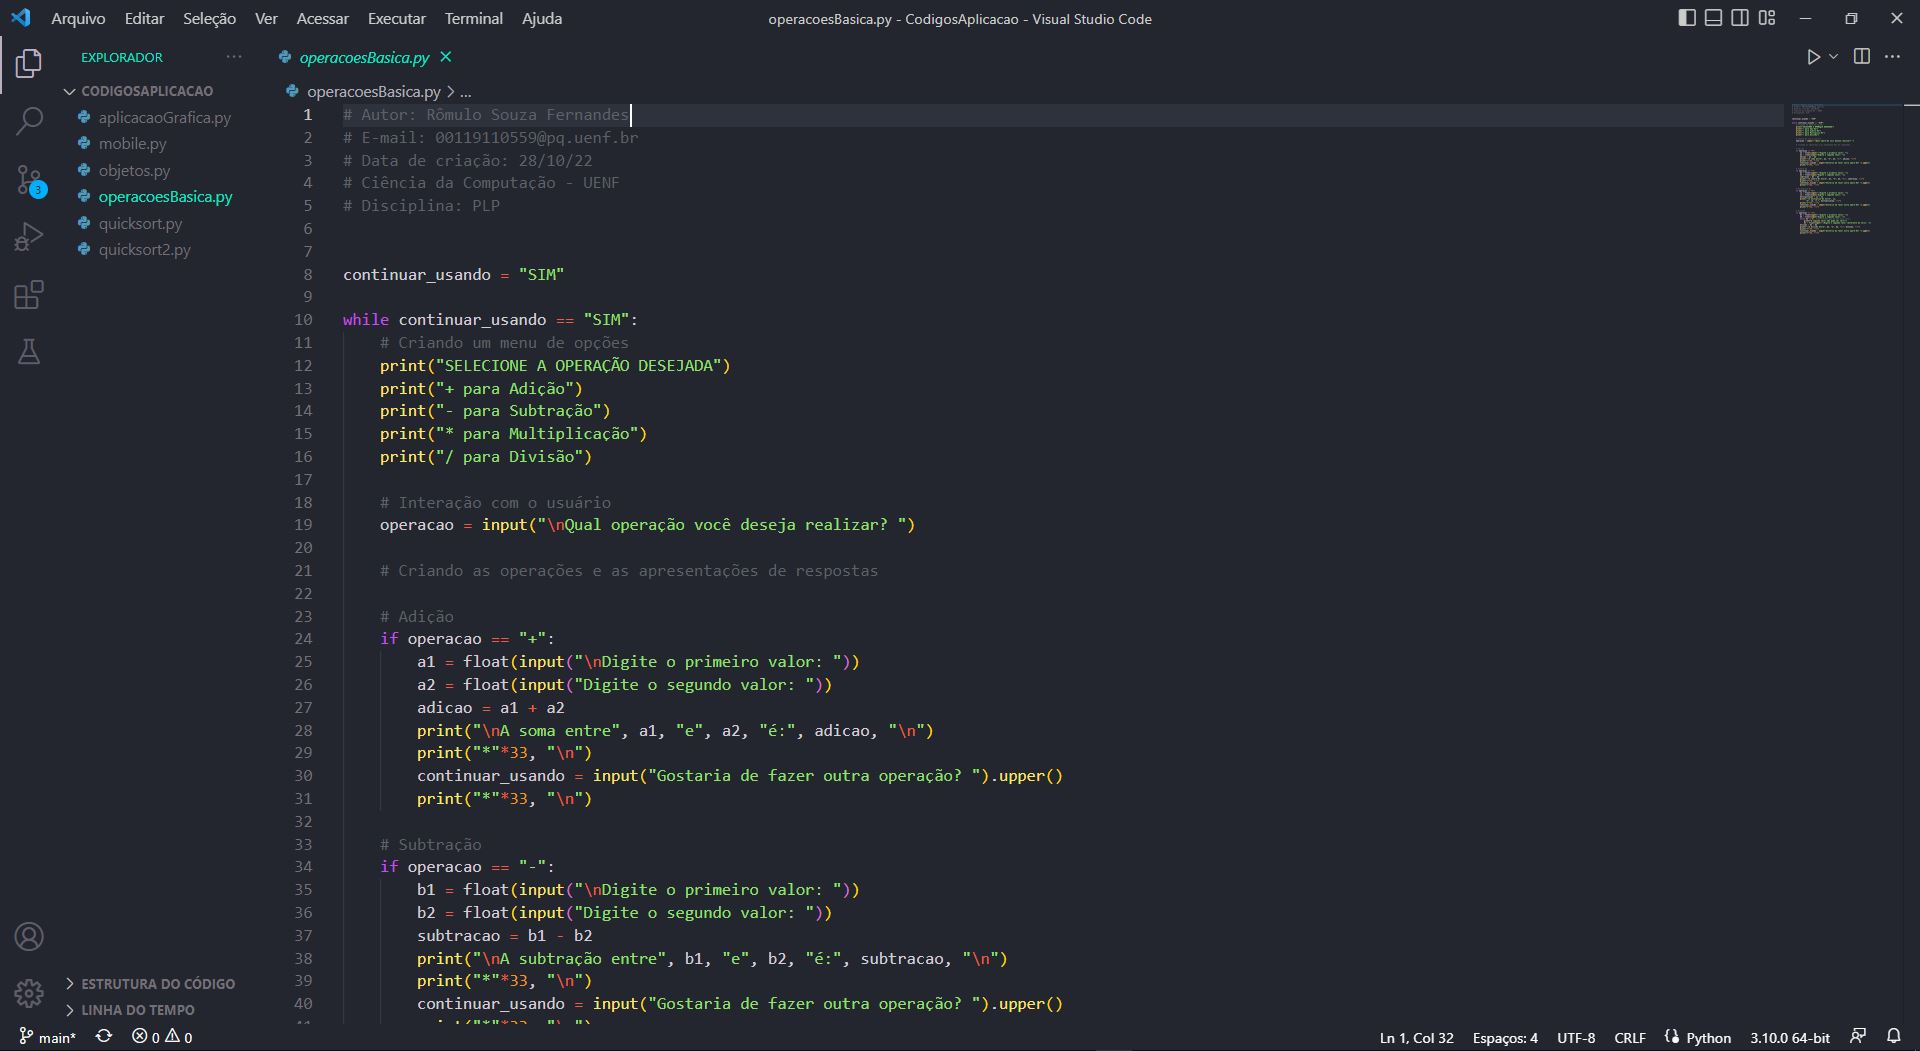
\includegraphics[width=12cm]{operacaocode.JPG} \\
			{\tiny \sf Fonte:{ Autor}}
		\end{center}
	\end{figure}
	
	\begin{figure}[H]
		\begin{center}
			\caption{Opção adição} \label{ling1}
			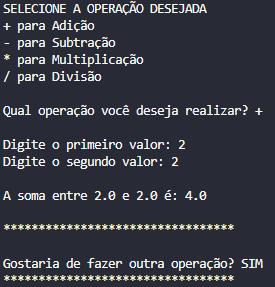
\includegraphics[width=5cm]{soma.PNG} \\
			{\tiny \sf Fonte:{ Autor}}
		\end{center}
	\end{figure}

	\begin{figure}[H]
		\begin{center}
			\caption{Opção subtração} \label{ling1}
			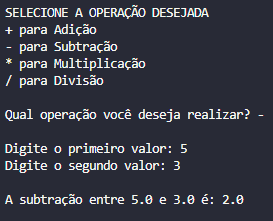
\includegraphics[width=5cm]{subtracao.PNG} \\
			{\tiny \sf Fonte:{ Autor}}
		\end{center}
	\end{figure}

	\begin{figure}[H]
		\begin{center}
			\caption{Opção multiplicação} \label{ling1}
			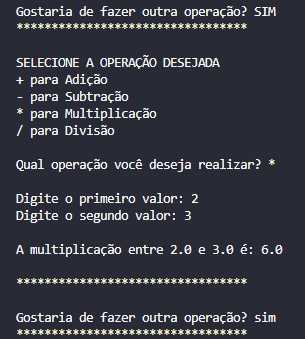
\includegraphics[width=5cm]{multi.PNG} \\
			{\tiny \sf Fonte:{ Autor}}
		\end{center}
	\end{figure}
	
	\begin{figure}[H]
		\begin{center}
			\caption{Opção divisão} \label{ling1}
			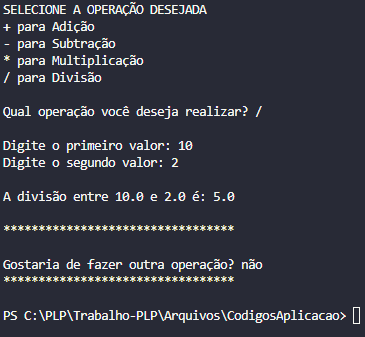
\includegraphics[width=5cm]{divisao.PNG} \\
			{\tiny \sf Fonte:{ Autor}}
		\end{center}
	\end{figure}
	
	
    \section{Programas gráficos}
     A seguir temos um exemplo de programa gráfico que é possível desenvolver utilizando a linguagem de programação Python e um framework chamado Tkinter. O Tkinter é uma biblioteca da linguagem Python, o mesmo vem instalado no pacote padrão de instalação do Python. Permitindo que qualquer computador que possua o interpretador Python instalado consiga desenvolver interfaces gráficas.
	\begin{lstlisting}
# Autor: Romulo Souza Fernandes
# E-mail: 00119110559@pq.uenf.br
# Data de criacao: 28/10/22
# Ciencia da Computacao - UENF
# Disciplina: PLP


# Importando todo conteudo do Tkinter
from tkinter import *

# Classe que exibe os controles na tela


class Application:
	def __init__(self, master=None):
		# Criacao do primeiro container, chamado widget1
		self.widget1 = Frame(master)
		# Informando o gerenciador de geometria pack
		self.widget1.pack()
		# Utilizando o widget label para imprimir na tela
		self.msg = Label(self.widget1, text="Romulo 
		Fernandes - UENF")
		self.msg["font"] = ("Verdana", "10", "italic",
		 "bold")
		self.msg.pack()
		self.sair = Button(self.widget1)
		self.sair["text"] = "Sair"
		self.sair["font"] = ("Calibri", "10")
		self.sair["width"] = 5
		self.sair["command"] = self.widget1.quit
		self.sair.pack()


# Instanciando a classe TK()
# Ela permite que os widgets sejam utilizados na aplicacao
root = Tk()

# Passando a variavel root como parametro do metodo
# construtor da classe Application
Application(root)

# Chamada do metodo para exibir na tela
root.mainloop()
	\end{lstlisting}

	\begin{figure}[H]
		\begin{center}
			\caption{Aplicação gráfica no Visual Studio Code} \label{ling1}
			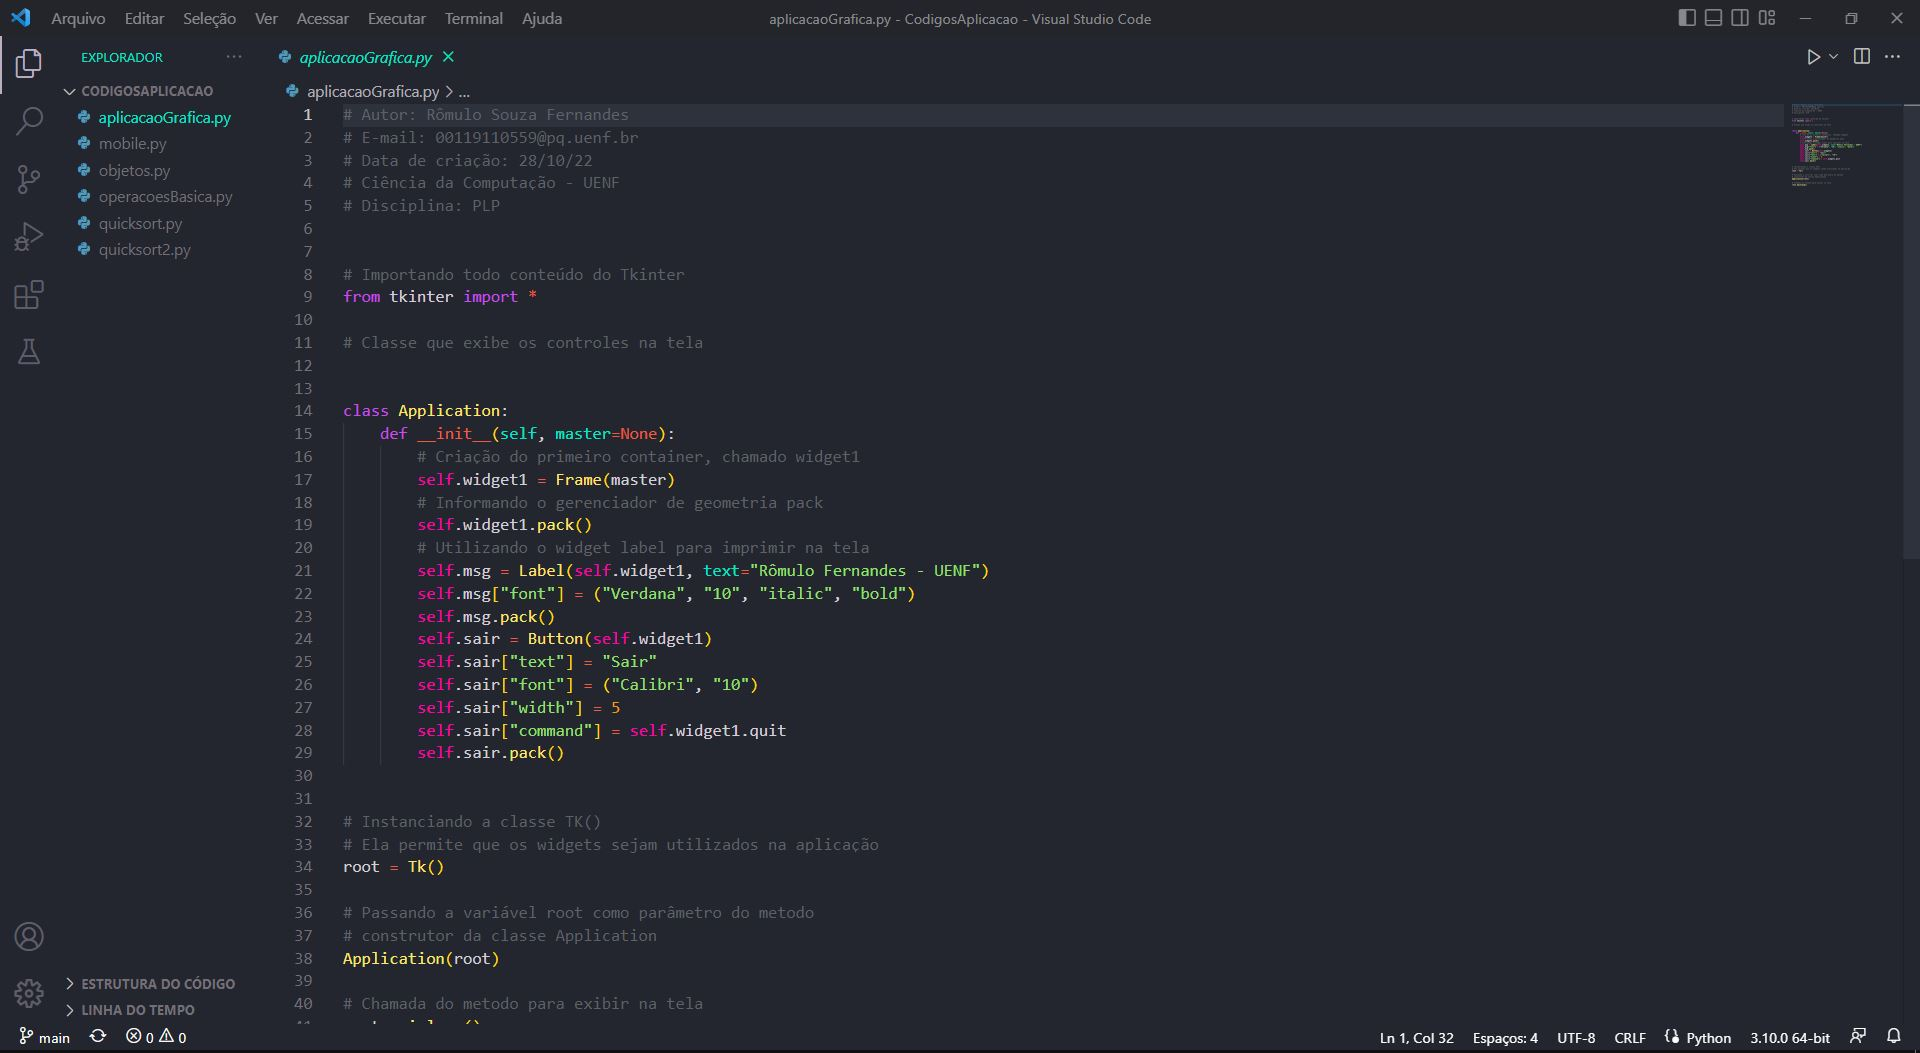
\includegraphics[width=15cm]{graficocode.JPG} \\
			{\tiny \sf Fonte:{ Autor}}
		\end{center}
	\end{figure}
	
	A seguir, uma imagem demonstrando o programa gráfico rodando no Visual Studio Code.
	
	\begin{figure}[H]
		\begin{center}
			\caption{Janela criada após a execução do código} \label{ling1}
			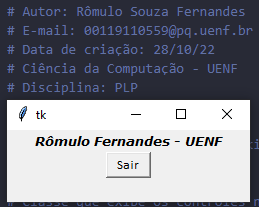
\includegraphics[width=7cm]{grafico.PNG} \\
			{\tiny \sf Fonte:{ Autor}}
		\end{center}
	\end{figure}

    \section{Programas com Objetos}
    Como sabemos, a Programação Orientada a Objetos (POO) é um dos paradigmas da linguagem
    Python, com base no conceito de classes e objetos. Abaixo temos um exemplo de código usando objetos na linguagem de programação Python.
\begin{lstlisting}
# Autor: Romulo Souza Fernandes
# E-mail: 00119110559@pq.uenf.br
# Data de criacao: 28/10/22
# Ciencia da Computacao - UENF
# Disciplina: PLP

# Definindo a Classe pessoa
class Pessoa:
	# Construtor
	def __init__(self, nome: str, idade: int, altura: float):
		self.nome = nome
		self.idade = idade
		self.altura = altura

	# Definindo o metodo dizer_ola()
	def dizer_ola(self):
		print(f'Ola, meu nome e {self.nome}. Tenho 
		{self.idade} 'f'anos e minha altura e {self.
		altura}m.')

	# Definindo o metodo cozinhar()
	def cozinhar(self, receita: str):
	print(f'Estou cozinhando um(a): {receita}')

	# Definindo o metodo andar()
	def andar(self, distancia: float):
	print(f'Sai para andar. Volto quando completar 
	{distancia} metros')


# Instancia um objeto da Classe "Pessoa"
pessoa = Pessoa(nome='Romulo', idade=22, altura=1.77)

# Chama os metodos de "Pessoa"
pessoa.dizer_ola()
pessoa.cozinhar('Sopa')
pessoa.andar(1200)
\end{lstlisting}
	Iniciamos definindo a classe pessoa, informando ao Python que as definições para a nova classe serão criadas. Logo temos o \textunderscore\textunderscore init \textunderscore\textunderscore, é um método construtor, sendo chamado ao instanciar objetos, é nesse método que os atributos do objeto são setados. Após, vem a definição dos métodos dizer\textunderscore ola(), cozinhar e andar(). No método dizer\textunderscore ola() é referenciado os atributos do próprio objeto. O método construtor \textunderscore\textunderscore init \textunderscore\textunderscore, é chamado quando "pessoa = Pessoa()", passando nome, idade e altura como parâmetro.
	
	\begin{figure}[H]
		\begin{center}
			\caption{Aplicação orientada a objetos no Visual Studio Code} \label{ling1}
			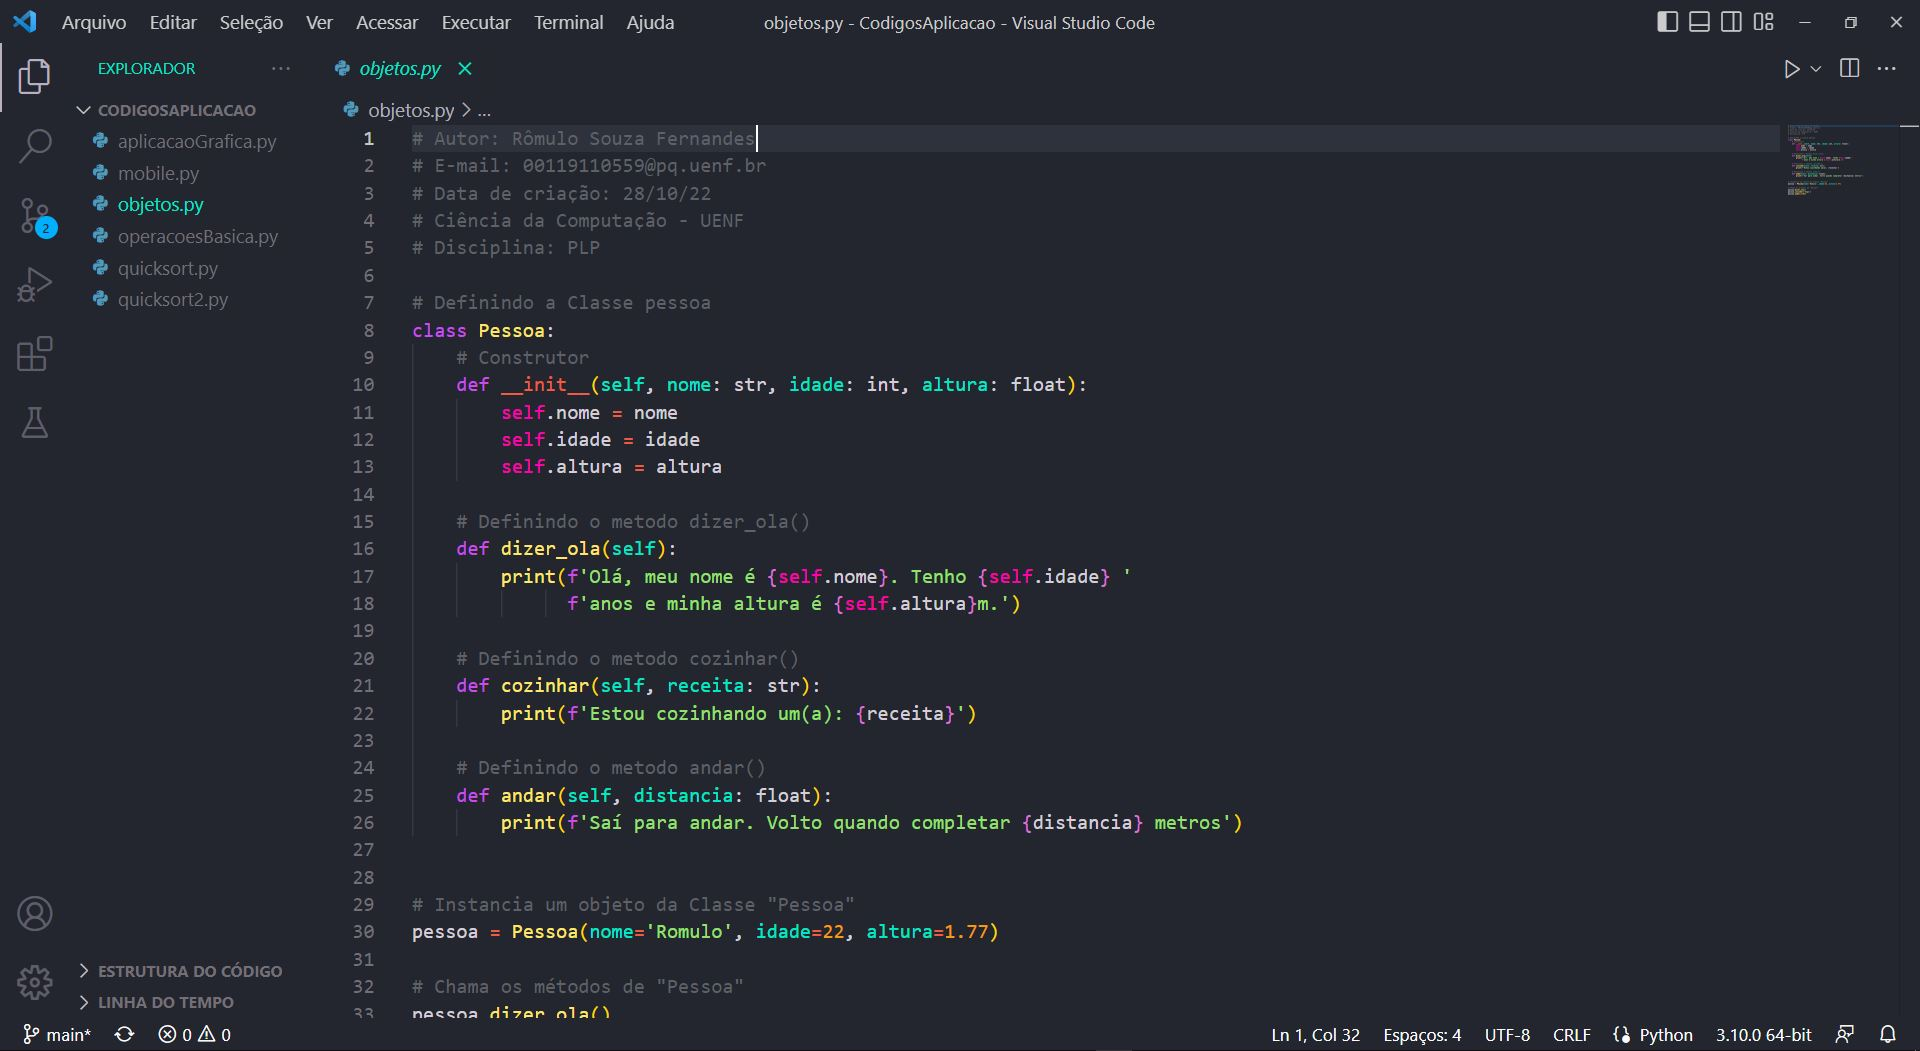
\includegraphics[width=15cm]{objetoscode.JPG} \\
			{\tiny \sf Fonte:{ Autor}}
		\end{center}
	\end{figure}
	
	A seguir temos uma imagem demonstrando o código utilizando objetos no Python, rodando no Visual Studio Code.
    \begin{figure}[H]
    	\begin{center}
    		\caption{Resultado após a compilação do código} \label{ling1}
    		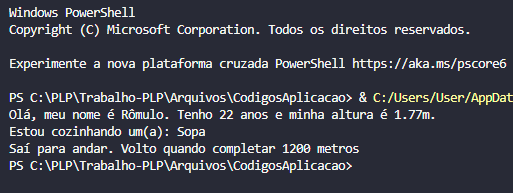
\includegraphics[width=9cm]{objetos.png} \\
    		{\tiny \sf Fonte:{ Autor}}
    	\end{center}
    \end{figure}
    
    
    \section{Quicksort}
    O código a seguir apresenta o algoritmo Quicksort no Python. O Quicksort funciona escolhendo um elemento como pivô e dividindo o array dado. Existem diversas versões de Quicksort que escolhem pivô de diferentes modos.
    \begin{itemize}
    	\item Sempre escolher o primeiro elemento do pivô.
    	\item Sempre escolher o último elemento do pivô.
    	\item Escolher um elemento aleatório.
    	\item Escolher a mediana como pivô
    \end{itemize}
	Nesse algoritmo está sendo utilizado o último elemento como pivô. Funcionando da seguinte forma, dado um array e um elemento X do array como um pivô, colocando X na posição correta em um array ordenado e coloca os outros elementos menores que o X antes do mesmo e os elementos maiores depois do X, todo esse processo sendo realizado em tempo linear.
\begin{lstlisting}
# Autor: Romulo Souza Fernandes
# E-mail: 00119110559@pq.uenf.br
# Data de criacao: 28/10/22
# Ciencia da Computacao - UENF
# Disciplina: PLP

# Programa Python para implementacao do Quicksort Sort

# Esta implementacao utiliza o pivo como o ultimo elemento na 
# lista
# Possui um ponteiro para acompanhar os elementos menores que o 
# pivo
# No final da funcao partition(), o ponteiro e trocado 
# pelo pivo para chegar a um numero "ordenado" relativo ao pivo


# Funcao para encontrar a posicao da particao
def partition(array, low, high):

	# Escolhe o elemento mais a direita como pivo
	pivot = array[high]

	# Ponteiro para o elemento maior
	i = low - 1

	# Percorre todos os elementos
	# Compara cada elemento com pivo
	for j in range(low, high):
		if array[j] <= pivot:

			# Se o elemento menor que o pivo for 
			# encontrado troca com o elemento 
			# maior apontado por i
			i = i + 1

			# Trocando elemento em i com elemento 
			# em j
			(array[i], array[j]) = (array[j], array
			[i])

	# Troca o elemento pivo pelo elemento maior especificado 
	# por i
	(array[i + 1], array[high]) = (array[high], array[i +
	 1])

	# Retorna a posicao de onde a particao e feita
	return i + 1

# Funcao para executar quicksort
def quickSort(array, low, high):
	if low < high:

	# Encontra o elemento pivo tal que
	# elemento menor que pivo esta a esquerda
	# elemento maior que pivo esta a direita
	pi = partition(array, low, high)

	# Chamada recursiva a esquerda do pivo
	quickSort(array, low, pi - 1)

	# Chamada recursiva a direita do pivo
	quickSort(array, pi + 1, high)


data = [1, 7, 4, 1, 10, 9, -2]
print("Array nao ordenado")
print(data)

size = len(data)

quickSort(data, 0, size - 1)

print('Array ordenado em ordem crescente:')
print(data)
\end{lstlisting}

\begin{figure}[H]
	\begin{center}
		\caption{Quicksort no Visual Studio Code} \label{ling1}
		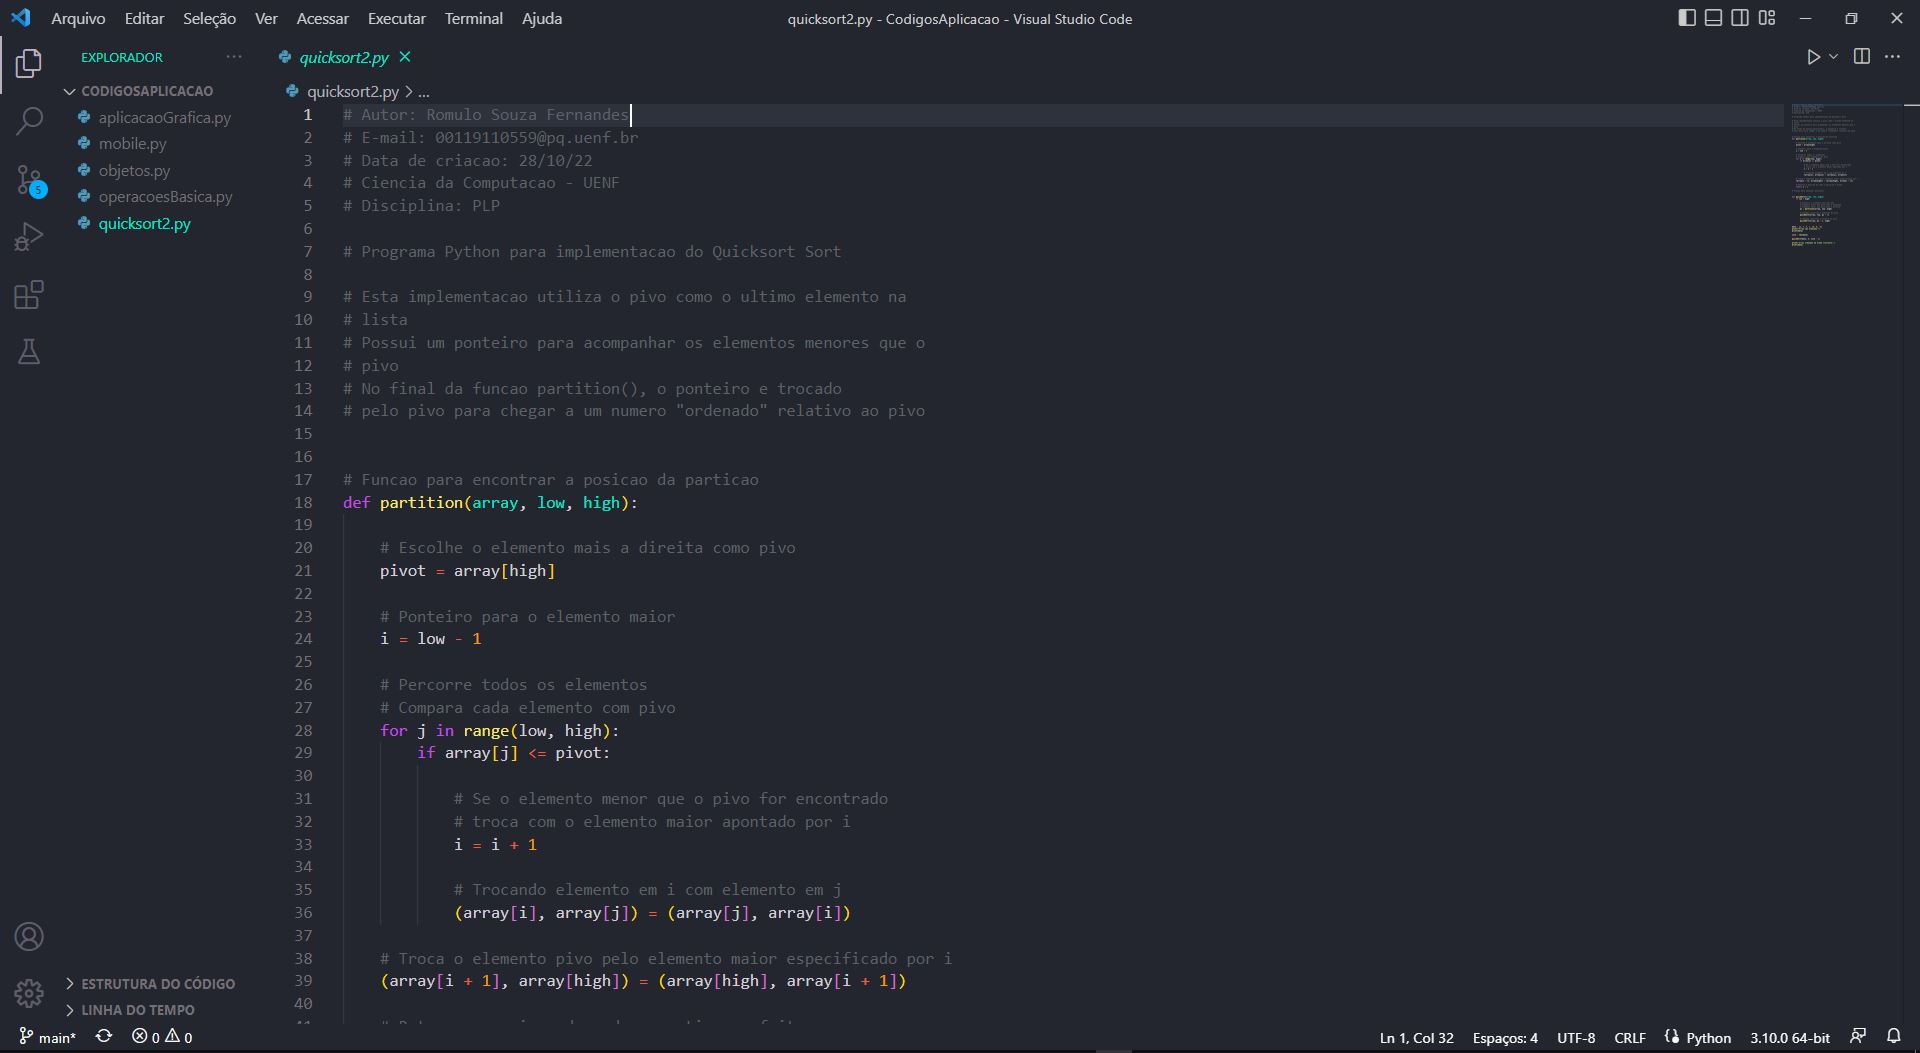
\includegraphics[width=15cm]{quickcode.JPG} \\
		{\tiny \sf Fonte:{ Autor}}
	\end{center}
\end{figure}

	A seguir temos uma imagem demonstrando o código Quicksort rodando no Visual Studio Code.
	\begin{figure}[H]
		\begin{center}
			\caption{Resultado da execução do código} \label{ling1}
			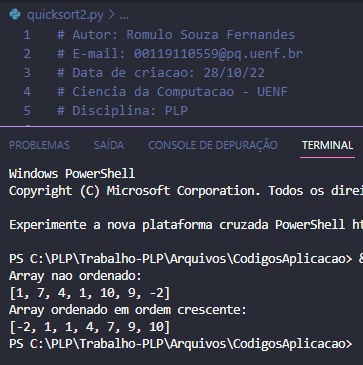
\includegraphics[width=7cm]{quick.PNG} \\
			{\tiny \sf Fonte:{ Autor}}
		\end{center}
	\end{figure}


    \section{Mobile}
    O código a seguir apresenta um programa com o objetivo de desenvolver um aplicativo para a plataforma mobile. Para isso foi utilizado a biblioteca Kivy, é bem completa para esse objetivo de desenvolvimento de aplicativos mobile e desktop em Python, tendo suporte para os seguintes sistemas operacionais: Android, IOS, Windows e OSX, com apenas 1 código. A biblioteca segue o padrão de UI chamado de NUI, que significa Natural User Interface, que é o padrão das aplicações que usamos rotineiramente em nossos celulares e PCs. Necessita apenas de uma simples instalação, usando o comando \textit{pip install kivy}.

 
    
    
    \begin{lstlisting}
# Autor: Romulo Souza Fernandes
# E-mail: 00119110559@pq.uenf.br
# Data de criacao: 28/10/22
# Ciencia da Computacao - UENF
# Disciplina: PLP

import kivy
from kivy.app import App
from kivy.uix.label import Label
from kivy.uix.boxlayout import BoxLayout

from kivy.uix.button import Button

kivy.require('1.9.1')

var = 0

def soma_um(instance):
	global var
	var += 1
	instance.text = str(var)


class MeuApp(App):
	def build(self):
		layout = BoxLayout(orientation='vertical',
		padding=[40, 20, 40, 20])

		layout.add_widget(Label(text='Romulo 
		Fernandes'))
		btn = Button(text='Pressione aqui', size=(100,
		50))

		btn.bind(on_press=soma_um)
		layout.add_widget(btn)
		return layout

if __name__ == '__main__':
	MeuApp().run()
    \end{lstlisting}

\begin{figure}[H]
	\begin{center}
		\caption{Aplicação mobile no Visual Studio Code} \label{ling1}
		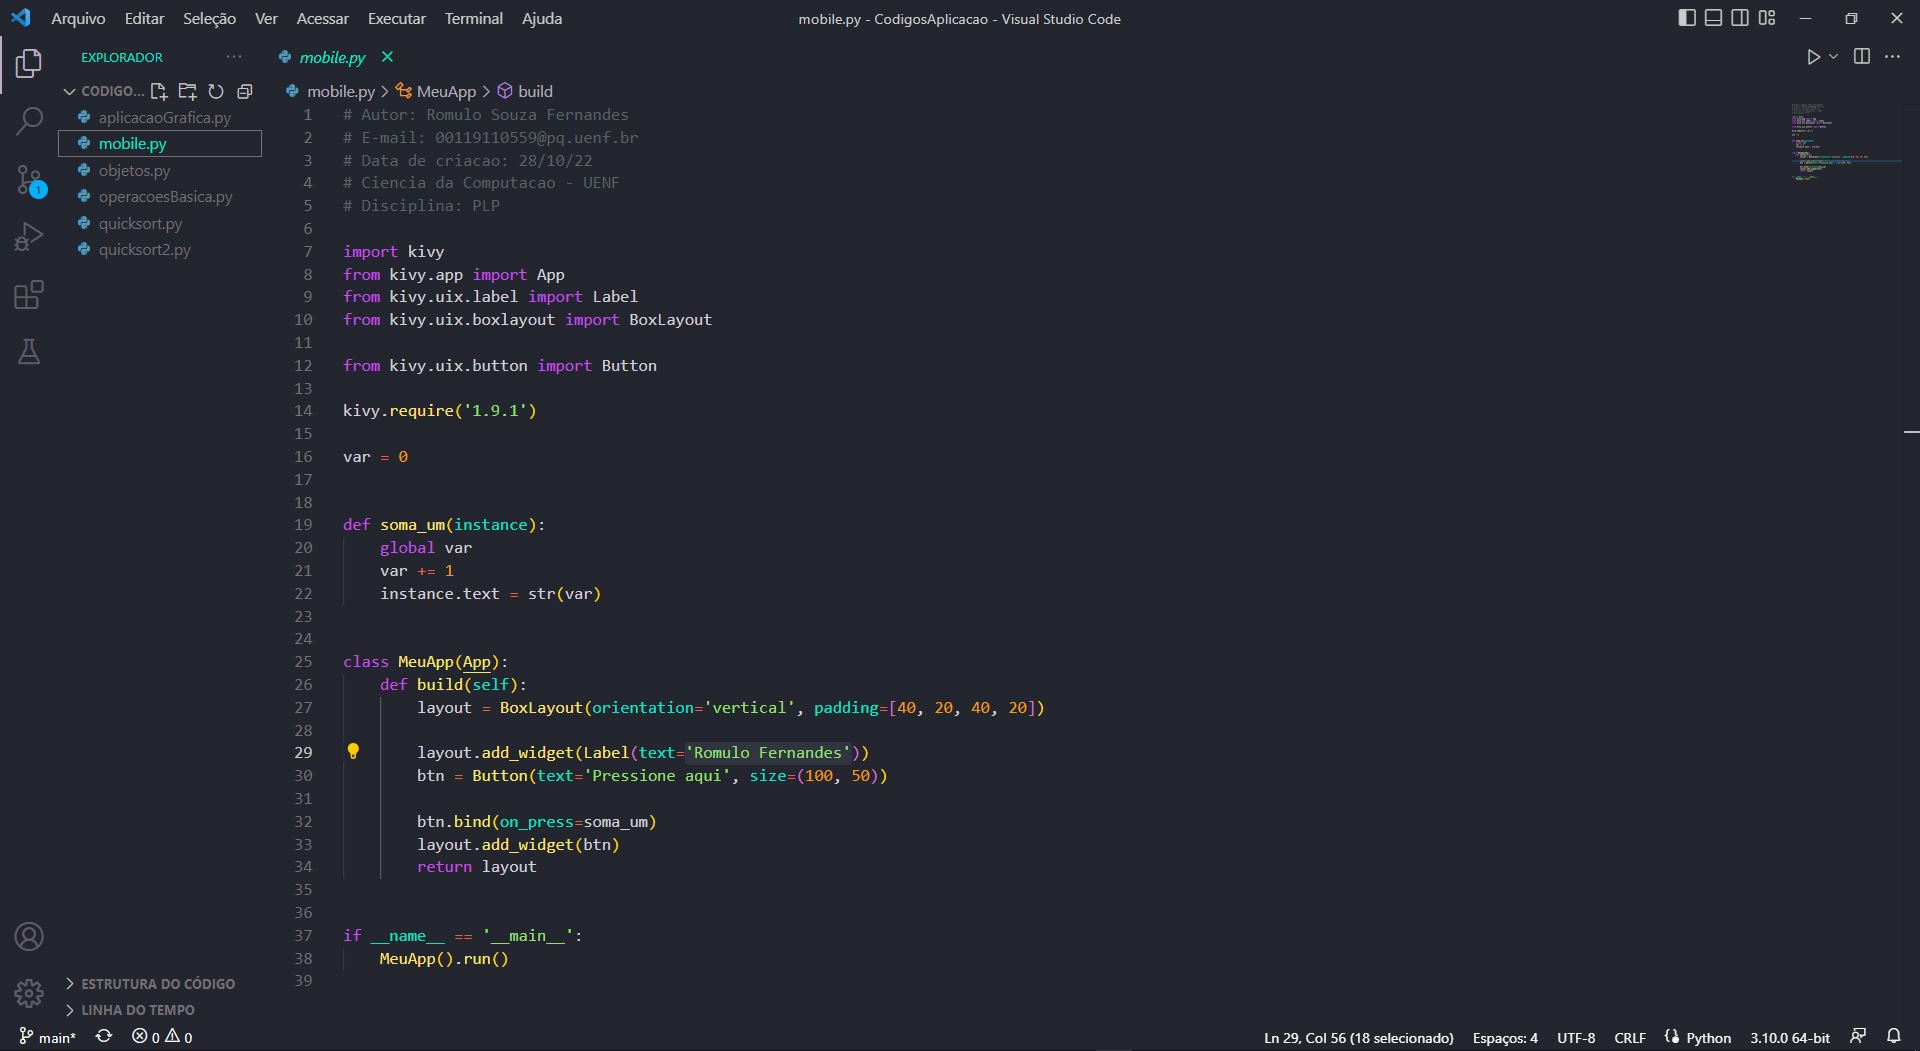
\includegraphics[width=15cm]{mobilecode.JPG} \\
		{\tiny \sf Fonte:{ Autor}}
	\end{center}
\end{figure}

	A seguir temos algumas imagens demonstrando o código da aplicação mobile rodando no Visual Studio Code.
	
		\begin{figure}[H]
		\begin{center}
			\caption{Janela criada com a execução do código} \label{ling1}
			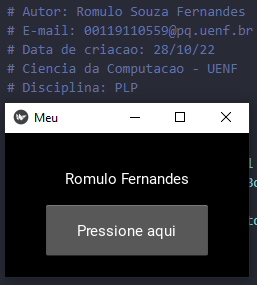
\includegraphics[width=9cm]{mobile.PNG} \\
			{\tiny \sf Fonte:{ Autor}}
		\end{center}
		\end{figure}

\begin{figure}[H]
	\begin{center}
		\caption{Tela 1 após executar o Kivy no celular} \label{ling1}
		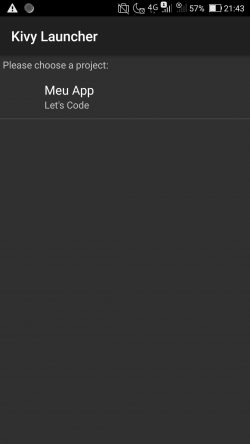
\includegraphics[width=5cm]{1mobile.JPG} \\
		{\tiny \sf Fonte:{ Autor}}
	\end{center}
\end{figure}

\begin{figure}[H]
	\begin{center}
		\caption{Tela 2 após executar o Kivy no celular} \label{ling1}
		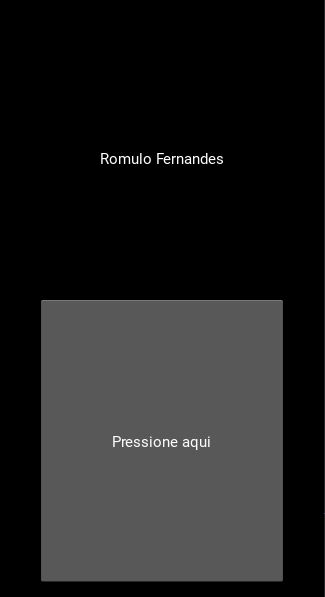
\includegraphics[width=5cm]{2mobile.JPG} \\
		{\tiny \sf Fonte:{ Autor}}
	\end{center}
\end{figure}
% Prof. Dr. Ausberto S. Castro Vera
% UENF - CCT - LCMAT - Curso de Ci\^{e}ncia da Computa\c{c}\~{a}o
% Campos, RJ,  2022
% Disciplina: Paradigmas de Linguagens de Programa\c{c}\~{a}o
% Aluno: Rômulo Souza Fernandes


\chapter{Ferramentas existentes e utilizadas}

Neste capítulo será apresentadas algumas ferramentas para auxiliar no desenvolvimento em Python, algumas dessas ferramentas foram utilizadas até mesmo para realizar esse trabalho. A seguir algumas ferramentas separadas por categoria.
\begin{itemize}
  \item Nome da ferramenta (compilador-interpretador)
  \item Endere\c{c}o na Internet
  \item Vers\~{a}o atual e utilizada
  \item Descri\c{c}\~{a}o simples (m\'{a}x 2 par\'{a}grafos)
  \item Telas capturadas da ferramenta
  \item Outras informa\c{c}\~{o}es
\end{itemize}

    \section{Notepad++}
	O Notepad++ é um editor de texto de código aberto funcional e gratuito, reconhecendo diversas linguagens de programação, uma delas é o Python. Sua última versão lançada é a Notepad++ v8.4.7, que está disponível para download gratuitamente no seu site oficial, o link a seguir fará o redirecionamento para a aba de downloads do \href{https://notepad-plus-plus.org/downloads/}{Notepad++}. 
	
    \section{Compilador XYZ}


    \section{Interpretador Shell}
	%https://docs.python.org/pt-br/3/tutorial/interpreter.html
	%https://education.ti.com/html/webhelp/EG_TINspire/PT/Subsystems/EG_Python/Content/m_workspaces/ws_shell.HTML

    \section{Ambientes de Programação IDE PyCharm e Visual Studio Code}
    
    \section{Debug}
     

\chapterimage{Conclusao.jpg} % Chapter heading image
% Prof. Dr. Ausberto S. Castro Vera
% UENF - CCT - LCMAT - Curso de Ci\^{e}ncia da Computa\c{c}\~{a}o
% Campos, RJ,  2022
% Disciplina: Paradigmas de Linguagens de Programa\c{c}\~{a}o
% Aluno: Rômulo Souza Fernandes


\chapter{Conclusões}

O desenvolvimento desse trabalho sobre Python, mesmo que de forma resumida, foi muito proveitoso em diversos aspectos, após a finalização do trabalho, é notável o ganho de conhecimento sobre a linguagem de programação Python, como sua história, diversas bibliotecas nativas, ferramentas de desenvolvimento como PyCharm, Visual Studio Code e Notepad++, várias áreas de aplicação da linguagem, paradigmas que a linguagem suporta e sua sintaxe. Além do ganho de conhecimento sobre a criação de arquivos usando o TeXstudio, editor de LaTeX, JabRef para fazer as referências bibliográficas e o LaTeX em si.

No decorrer do desenvolvimento deste trabalho surgiram algumas dificuldades, como a falta de material para basear o trabalho, como por exemplo livros disponibilizados apenas para compra ou visualização teste, oferecendo apenas algumas páginas. Além de artigos em outras línguas, que gerou alguns problemas na tradução de termos técnicos, favorecendo a demora no desenvolvimento do trabalho. Apesar de todas as dificuldades, foi possível tirar proveito, gerando conhecimento sobre novas ferramentas e meios de pesquisa de artigos bibliográficos, livros, entre outros canais de informações. Além de aprender novos termos técnicos, que são muito pertinentes na área de Ciência da Computação.

Alguns pontos não considerados que poderiam ser estudados e acrescentados nesse trabalho são:





\chapterimage{Bibliografia.png}
\bibliographystyle{alpha}
\bibliography{PythonBib}
\addcontentsline{toc}{chapter}{\textcolor{ocre}{Bibliografia}}
%----------------------------------------------------------------------------------------
%	INDEX
%----------------------------------------------------------------------------------------

\cleardoublepage
\phantomsection
\setlength{\columnsep}{0.75cm}
\addcontentsline{toc}{chapter}{\textcolor{ocre}{Index}}
\printindex

%----------------------------------------------------------------------------------------
% Prof. Dr. Ausberto S. Castro Vera
% UENF - CCT - LCMAT - Curso de Ci\^{e}ncia da Computa\c{c}\~{a}o
% Campos, RJ,  2022
% Disciplina: Paradigmas de Linguagens de Programa\c{c}\~{a}o
% Aluno: Rômulo Souza Fernandes




\noindent
\textbf{Disciplina:} \textit{Paradigmas de Linguagens de Programa\c{c}\~{a}o 1970}\\
\textbf{Linguagem:} \textit{LinguagemXYZabcd}\\
\textbf{Aluno:} \textit{ \color{blue} Rômulo Souza Fernandes}


\section*{Ficha de avalia\c{c}\~{a}o:}



\begin{tabular}{|p{12cm}|c|}
  \hline
  % after \\: \hline or \cline{col1-col2} \cline{col3-col4} ...
  \textbf{Aspectos de avalia\c{c}\~{a}o (requisitos m\'{\i}nimos)} & \textbf{Pontos} \\
  \hline
   \color{red} Introdu\c{c}\~{a}o (M\'{a}ximo: 01 pontos) &  \\
  $\bullet$ Aspectos hist\'{o}ricos &  \\
  $\bullet$ \'{A}reas de Aplica\c{c}\~{a}o da linguagem &  \\
  \hline
 \color{red}  Elementos b\'{a}sicos da linguagem (M\'{a}ximo: 01 pontos) &  \\
  $\bullet$ Sintaxe (vari\'{a}veis, constantes, comandos, opera\c{c}\~{o}es, etc.) &  \\
  $\bullet$ Cada elemento com exemplos (c\'{o}digo e execu\c{c}\~{a}o) &  \\
  \hline
  \color{red} Aspectos Avan\c{c}ados da linguagem (M\'{a}ximo: 2,0 pontos) &  \\
  $\bullet$ Sintaxe (vari\'{a}veis, constantes, comandos, opera\c{c}\~{o}es, etc.) &  \\
  $\bullet$ Cada elemento com exemplos (c\'{o}digo e execu\c{c}\~{a}o) &  \\
  $\bullet$ Exemplos com fonte diferenciada (listing) & \\
  \hline
  \color{red} M\'{\i}nimo 5 Aplica\c{c}\~{o}es completas - Aplica\c{c}\~{o}es (M\'{a}ximo : 2,0 pontos) &  \\
  $\bullet$ Uso de rotinas-fun\c{c}\~{o}es-procedimentos, E/S formatadas &  \\
  $\bullet$ Uma Calculadora &  \\
  $\bullet$ Gr\'{a}ficos &  \\
  $\bullet$ Algoritmo QuickSort &  \\
  $\bullet$ Outra aplica\c{c}\~{a}o &  \\
  $\bullet$ Outras aplica\c{c}\~{o}es ... &  \\
  \hline
  \color{red} Ferramentas (compiladores, interpretadores, etc.) (M\'{a}ximo : 1,0 pontos) &  \\
  $\bullet$ Ferramentas utilizadas nos exemplos: pelo menos DUAS&  \\
  $\bullet$ Descri\c{c}\~{a}o de Ferramentas existentes:  m\'{a}ximo 5&  \\
  $\bullet$ Mostrar as telas dos exemplos junto ao compilador-interpretador&  \\
  $\bullet$ Mostrar as telas dos resultados com o uso das ferramentas &  \\
  $\bullet$ Descri\c{c}\~{a}o das ferramentas (autor, vers\~{a}o, homepage, tipo, etc.) &  \\
  \hline
  \color{red} Organiza\c{c}\~{a}o do trabalho (M\'{a}ximo: 01 ponto) &  \\
  $\bullet$ Conte\'{u}do, Historia, Se\c{c}\~{o}es, gr\'{a}ficos, exemplos, conclus\~{o}es, bibliografia &  \\
  $\bullet$ Cada elemento com exemplos (c\'{o}digo e execu\c{c}\~{a}o, ferramenta, nome do aluno) &  \\
  \hline
  \color{red} Uso de Bibliografia (M\'{a}ximo: 01 ponto)&  \\
   $\bullet$ Livros: pelo menos 3&  \\
   $\bullet$ Artigos cient\'{\i}ficos: pelo menos 3 (IEEE Xplore, ACM Library)&  \\
   $\bullet$ Todas as Refer\^{e}ncias dentro do texto, tipo [ABC 04] & \\
   $\bullet$ Evite Refer\^{e}ncias da Internet & \\
   \hline
     &  \\
  \color{red} Conceito do Professor (Opcional: 01 ponto) & \\
  \hline
   & \\
  \hfill \color{blue} Nota Final do trabalho: & \\
  \hline
\end{tabular}\\
\textit{Observa\c{c}\~{a}o:} Requisitos m\'{\i}nimos significa a \textit{metade} dos pontos


\end{document}

